% \special{dvipdfmx:config z 0}
\documentclass[UTF8,a4paper,AutoFakeBold,AutoFakeSlant]{article}
\usepackage[a4paper,left=2.8cm,right=2.6cm,top=3.7cm,bottom=3.5cm]{geometry}
\usepackage{ctex}
% \usepackage{xeCJK}
\usepackage{graphicx}
\usepackage{pythonhighlight}
\usepackage[mathscr]{eucal}
\usepackage{mathrsfs}
\usepackage{booktabs}
\usepackage{capt-of} 
\usepackage{hyperref} 
\usepackage{abstract}
\usepackage{amsmath}
\usepackage{listings}
\usepackage{color}
\usepackage{caption}
\usepackage{subfigure}
\usepackage{enumerate}
\usepackage{amsfonts} 
\usepackage{CJK,CJKnumb}
\usepackage{float}
% \usepackage{gbt7714}
\usepackage{framed}
\usepackage{multirow}
\usepackage{animate}
\usepackage[framemethod=tikz]{mdframed}


\newcommand{\song}{\CJKfamily{song}}    % 宋体   (Windows自带simsun.ttf)
\newcommand{\fs}{\CJKfamily{fs}}        % 仿宋体 (Windows自带simfs.ttf)
\newcommand{\kai}{\CJKfamily{kai}}      % 楷体   (Windows自带simkai.ttf)
\newcommand{\hei}{\CJKfamily{hei}}      % 黑体   (Windows自带simhei.ttf)
\newcommand{\li}{\CJKfamily{li}}        % 隶书   (Windows自带simli.ttf) 
\newcommand{\ssong}{\CJKfamily{STSong}}

% \xeCJKsetup{SlantFactor = 0.3}
% % \xeCJKsetup{SlantFactor = -0.7}
\setCJKmainfont[BoldFont=SimHei, SlantedFont=KaiTi]{SimSun}



% -- 中文字体 --
%\setCJKmainfont{Microsoft YaHei}  % 微软雅黑
%\setCJKmainfont{YouYuan}  % 幼圆
%\setCJKmainfont{NSimSun}  % 新宋体
%\setCJKmainfont{KaiTi}    % 楷体
% \setCJKmainfont{SimSun}   % 宋体
%\setCJKmainfont{SimHei}   % 黑体
% \setCJKfamilyfont{hwsong}{STSong}
 
% -- 英文字体 --
% \setmainfont{Times New Roman}
% \setmainfont{DejaVu Sans}
% \setmainfont{Latin Modern Mono}
% \setmainfont{Consolas}
% \setmainfont{Courier New}


\usepackage{xcolor}  	%高亮使用的颜色
\definecolor{commentcolor}{RGB}{85,139,78}
\definecolor{stringcolor}{RGB}{206,145,108}
\definecolor{keywordcolor}{RGB}{34,34,250}
\definecolor{backcolor}{RGB}{220,220,220}


\definecolor{shadecolor}{rgb}{0.92,0.92,0.92}   %灰色引用背景色



\usepackage{accsupp}	
\newcommand{\emptyaccsupp}[1]{\BeginAccSupp{ActualText={}}#1\EndAccSupp{}}

\usepackage{listings}
\lstset{						%高亮代码设置
	language=python, 					%Python语法高亮
	linewidth=0.95\linewidth,      		%列表list宽度
	%basicstyle=\ttfamily,				%tt无法显示空格
	commentstyle=\color{commentcolor},	%注释颜色
	keywordstyle=\color{keywordcolor},	%关键词颜色
	stringstyle=\color{stringcolor},	%字符串颜色
	%showspaces=true,					%显示空格
	numbers=left,						%行数显示在左侧
	numberstyle=\tiny\emptyaccsupp,		%行数数字格式
	numbersep=5pt,						%数字间隔
	frame=single,						%加框
	framerule=0.1pt,						%划线
	escapeinside=@@,					%逃逸标志
	emptylines=1,						%
	xleftmargin=3em,					%list左边距
	backgroundcolor=\color{backcolor},	%列表背景色
	tabsize=4,							%制表符长度为4个字符
	% gobble=4							%忽略每行代码前4个字符
}




\renewcommand{\abstractname}{}    % clear the title
\renewcommand{\absnamepos}{empty}
%去除摘要两边缩进
\makeatletter
  \renewenvironment{abstract}{%
      \if@twocolumn
        \section*{\abstractname}%
      \else
        \small
        \begin{center}%
          {\bfseries \abstractname\vspace{-.5em}\vspace{\z@}}%
        \end{center}%
      \fi}
      {}
  \makeatother
  \lstset{
    language=Matlab,
    keywords={break,case,catch,continue,else,elseif,end,for,function,
       global,if,otherwise,persistent,return,switch,try,while},
    basicstyle=\ttfamily,
    keywordstyle=\color{blue}\bfseries,
    commentstyle=\color{dkgreen},
    stringstyle=\color{dkpurple},
    backgroundcolor=\color{white},
    tabsize=4,
    showspaces=false,
    showstringspaces=false
}

\title{\textbf{\textsf{{\textsf{HW} \heiti{机器学习概论}}}}} 
\author{\song PB19151769~~~~~马宇骁}
\date{}


\begin{document}

\maketitle

\tableofcontents
\newpage



% ----------------section分割线-------------------------------------------

\section{HW1}
\begin{figure}[htbp]
  \centering
  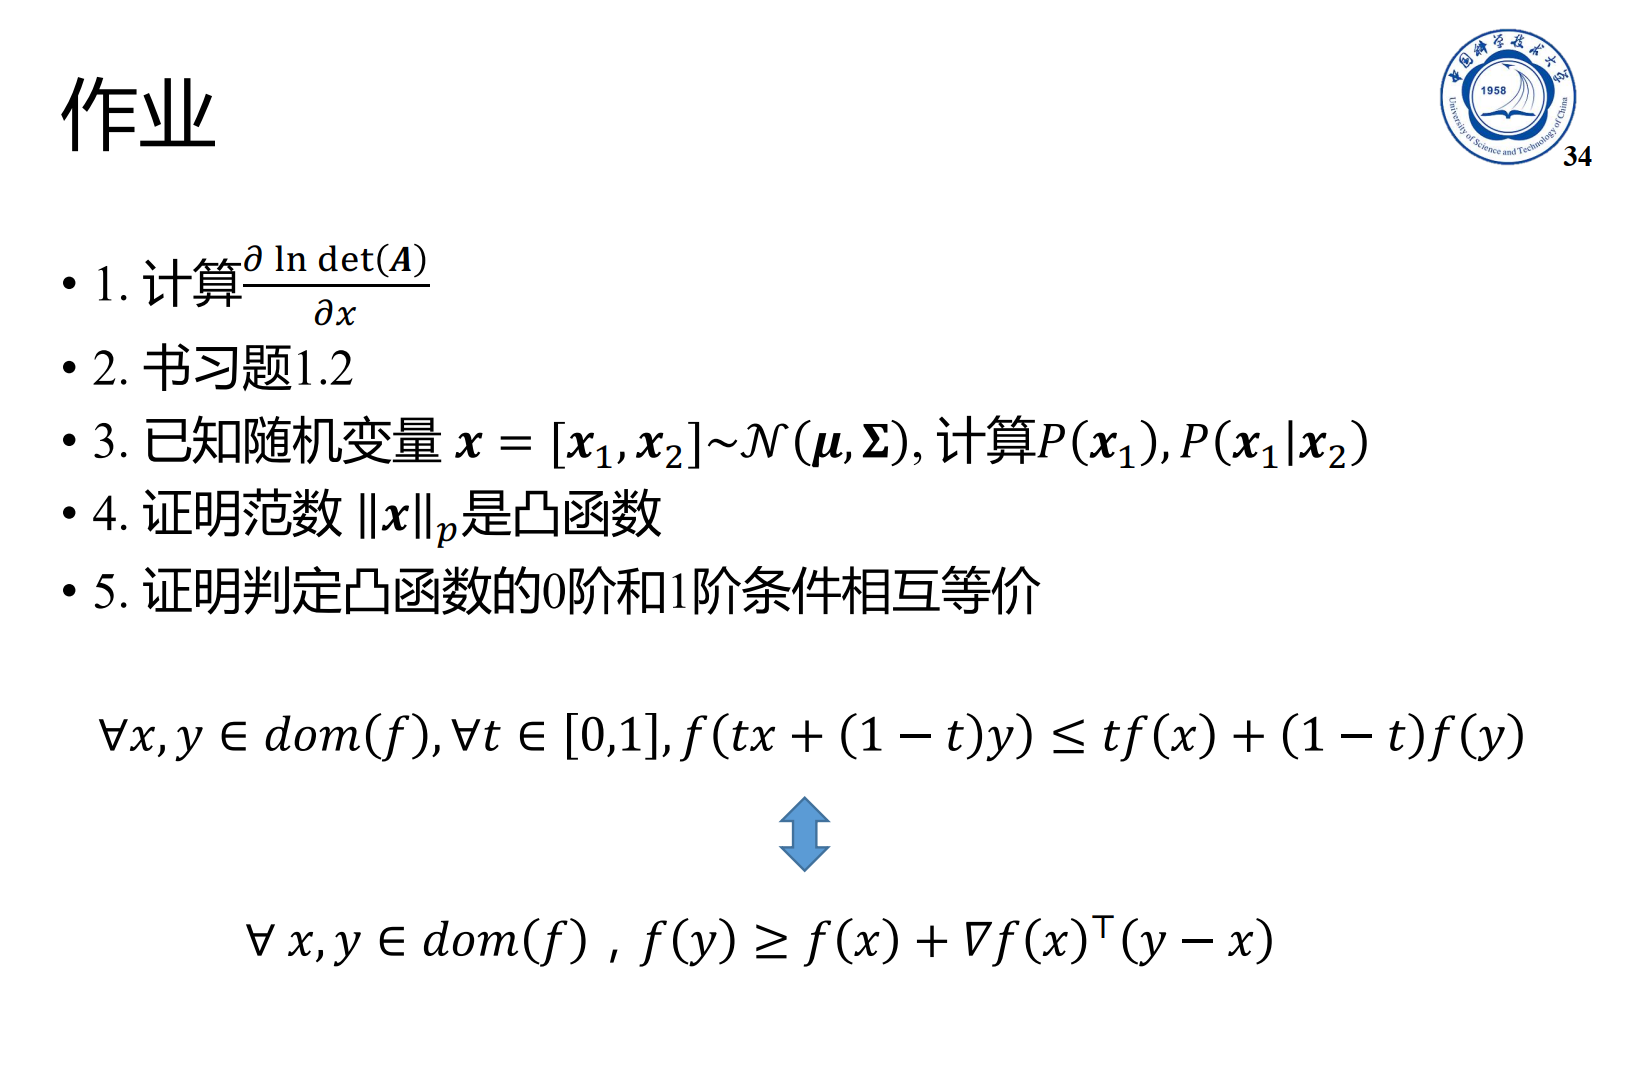
\includegraphics[scale=0.425]{hw1.png}
  % \caption{}
  \label{f1}
\end{figure}


\subsection{}
先由:
\begin{equation*}
  \frac{\partial \operatorname{det}(A)}{\partial A_{i j}}=\frac{\partial \sum_{k} A_{i k} \operatorname{adj}^{T}(A)_{i k}}{\partial A_{i j}}=\sum_{k} \frac{\partial A_{i k} \operatorname{adj}^{T}(A)_{i k}}{\partial A_{i j}} \\
  =\sum_{k} \frac{\partial A_{i k}}{\partial A_{i j}} \operatorname{adj}^{T}(A)_{i k}+\sum_{k} A_{i k} \frac{\partial \operatorname{adj}^{T}(A)_{i k}}{\partial A_{i j}}
\end{equation*}
其中,$ \frac{\partial \operatorname{adj}^{T}(A)_{i k}}{\partial A_{i j}} = 0 $,有:
\begin{equation*}
  \frac{\partial \operatorname{det}(A)}{\partial A_{i j}} = \sum_{k} \frac{\partial A_{i k}}{\partial A_{i j}} \operatorname{adj}^{T}(A)_{i k} = \operatorname{adj}^{T}(A)_{i j}
\end{equation*}
因此,
\begin{equation*}
  \begin{aligned}
    \frac{\partial \ln \operatorname{det}(A)}{\partial x} & = \frac{1}{\operatorname{det}(A)} \sum_{i, j} \frac{\partial \operatorname{det}(A)}{\partial A_{i j}} \frac{\partial A_{i j}}{\partial x} \\
                                                          & = \frac{1}{\operatorname{det}(A)} \sum_{i, j} \operatorname{adj}^{T}(A)_{i j} \frac{\partial A_{i j}}{\partial x}                         \\
                                                          & = \frac{1}{\operatorname{det}(A)} \sum_{i, j} \operatorname{adj}(A)_{j i} \frac{\partial A_{i j}}{\partial x}                             \\
                                                          & = \frac{1}{\operatorname{det}(A)} \sum_{j = 1}^{n}\left(A^{*} \frac{\partial A}{\partial x}\right)_{j j}                                  \\
                                                          & = \operatorname{tr}\left(A^{-1} \frac{\partial A}{\partial x}\right)
  \end{aligned}
\end{equation*}


\subsection{}
题中的表1.1如图\ref{f2}.
\begin{figure}[htbp]
  \centering
  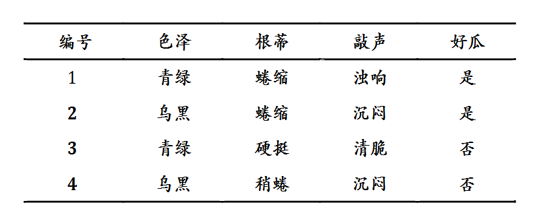
\includegraphics[scale=0.725]{1_2.png}
  \caption{西瓜数据集}
  \label{f2}
\end{figure}

由题可知:

仅从表中发现有3个因素,每个因素有2, 3, 3种取值,
假设空间总共有 $ 3\times4\times4 + 1 = 49 $ 种假设,其中有1种是空集,不考虑空时:

全部不泛化 $2\times3\times3=18$ 种假设

一个属性泛化:$2\times3+3\times3+2\times3=21$ 种假设

两个属性泛化:$2+3+3=8$ 种假设

三属性泛化:1种假设

用这48种假设的排列组合来组成析合范式,展开序列为:
\begin{equation*}
  1, C_{48}^{1}, C_{48}^{2}, \cdots ,C_{48}^{48}
\end{equation*}
共49个数,左边的1代表‘空’,一个都不选,右边的1代表全部选。

如果k=48,$2^{48} - 1$ 种 (排除一种都不选的情况).

如果0<k<48,$ \sum_{i=0}^k C_{48}^i-1 = \sum_{i=1}^k C_{48}^i $ 种.

(以上结果均需去重)

若k足够大,并考虑重复,则演变为在不泛化的18种中选择,共有$2^{18} – 1$种假设。


\subsection{}
令
\begin{equation*}
  \Sigma =
  \begin{pmatrix}
    \sigma_1^2                  & \operatorname{Cov}(x_1,x_2) \\
    \operatorname{Cov}(x_2,x_1) & \sigma_2^2
  \end{pmatrix}
\end{equation*}
其中,$ \rho = \frac{\operatorname{Cov}(x_1,x_2)}{\sigma_1 \sigma_2} $

由分布可知:
\begin{equation*}
  f\left(x_{1}, x_{2}\right)=\frac{1}{2 \pi\left(1-\rho^{2}\right)^{\frac{1}{2}} \sigma_{1} \sigma_{2}} e^{-\frac{1}{2\left(1-\rho^{2}\right)}\left[\left(\frac{x_{1}-\mu_{1}}{\sigma_{1}}\right)^{2}-2 \rho\left(\frac{x_{1}-\mu_{1}}{\sigma_{1}}\right)\left(\frac{x_{2}-\mu_{2}}{\sigma_{2}}\right)+\left(\frac{x_{2}-\mu_{2}}{\sigma_{2}}\right)^{2}\right]}
\end{equation*}

所以,
\begin{equation*}
  \begin{aligned}
    P(x_1) & = \int_{-\infty}^{x_1} \int_{-\infty}^{+\infty} f\left(x_{1}, x_{2}\right) \,\operatorname{d}x_2 \operatorname{d}x_1                                                                                                                                                                                                                                                                                                           \\
           & =  \int_{-\infty}^{x_1} \int_{-\infty}^{+\infty} \frac{1}{2 \pi\left(1-\rho^{2}\right)^{\frac{1}{2}} \sigma_{1} \sigma_{2}} e^{-\frac{1}{2\left(1-\rho^{2}\right)}\left[\left(\frac{x_{1}-\mu_{1}}{\sigma_{1}}\right)^{2}-2 \rho\left(\frac{x_{1}-\mu_{1}}{\sigma_{1}}\right)\left(\frac{x_{2}-\mu_{2}}{\sigma_{2}}\right)+\left(\frac{x_{2}-\mu_{2}}{\sigma_{2}}\right)^{2}\right]} \,\operatorname{d}x_2 \operatorname{d}x_1 \\
           & = \int_{-\infty}^{x_1} f_{x_1}(x_1) \operatorname{d}x_1                                                                                                                                                                                                                                                                                                                                                                        \\
           & = \int_{-\infty}^{x_1} \frac{1}{\sigma_1 \sqrt{2 \pi}} e^{-\frac{1}{2}\left(\frac{x-\mu_1}{\sigma_1}\right)^{2}} \operatorname{d}x_1
  \end{aligned}
\end{equation*}

\begin{equation*}
  \begin{aligned}
    P(x_1|x_2) & =  \int_{-\infty}^{x_1}  \frac{f(x_1,x_2)}{f_{x_2}(x_2)}  \operatorname{d}x_1                                                     \\
               & =  \int_{-\infty}^{x_1}  \frac{1}{\sqrt{2\pi}\sigma_1\sqrt{1-\rho^2}} e^{-\frac{(w-\rho v)^2}{2(1-\rho^2)}}   \operatorname{d}x_1
  \end{aligned}
\end{equation*}
其中,
\begin{equation*}
  w = \frac{(x_1-\mu_1)^2}{\sigma_1^2}, \, v = \frac{(x_2-\mu_2)^2}{\sigma_2^2}.
\end{equation*}


\subsection{}
p-范数($p \geq 1$):
\begin{equation*}
  f(X) = \left\lVert X\right\rVert_p  = (\sum_{i=1}^{n}X_i^p)^{\frac{1}{p}}
\end{equation*}
要证明$f$为凸函数,\\
及证明 $f(\lambda \mathbf{x}+(1-\lambda) \mathbf{y}) \leq \lambda f(\mathbf{x})+(1-\lambda) f(\mathbf{y})$ 对任意的$ 0 \leq \lambda \leq 1 $ 成立

由Minkowski 不等式可知:\\
设  S  是一个度量空间,  $1 \leq p \leq \infty$ , $f$, $g \in L^{p}(S)$  ,那么  $f+g \in L^{p}(S)$  ,我们有:
\begin{equation*}
  \|f+g\|_{p} \leq\|f\|_{p}+\|g\|_{p}
\end{equation*}
即,
\begin{equation*}
  \left(\sum_{i=1}^{n}\left(x_{i}+y_{i}\right)^{p}\right)^{\frac{1}{p}} \leq\left(\sum_{i=1}^{n} x_{i}^{p}\right)^{\frac{1}{p}}+\left(\sum_{i=1}^{n} y_{i}^{p}\right)^{\frac{1}{p}}
\end{equation*}
如果  $1<p<\infty$  ,等号成立当且仅当 $ k \geq 0$ , $f=k g$  或  $g=k f $

故,
\begin{equation*}
  \begin{aligned}
    \|\lambda \mathbf{x}+(1-\lambda) \mathbf{y}\|_{\mathrm{p}} & \leq\|\lambda \mathbf{x}\|+\|(1-\lambda) \mathbf{y}\|_{\mathrm{p}}         \\
                                                               & =\lambda\|\mathbf{x}\|_{\mathrm{p}}+(1-\lambda)\|\mathbf{y}\|_{\mathrm{p}}
  \end{aligned}
\end{equation*}
凸函数得证.


\subsection{}
\begin{itemize}
  \item 充分性
\end{itemize}

令 $ a = 1-t $, $ a \in \left[0, 1\right]  $,
\begin{equation*}
  \begin{aligned}
             & f(t x+(1-t) y) \leq t f(x)+(1-t) f(y)                                       \\
    \implies & a f(y) \geq f[(1-a) x+a y]-(1-a) f(x)=f[x+a(y-x)]+a f(x)-f(x)               \\
    \implies & f(y) \geq f(x)+\lim _{a \rightarrow 0} \frac{f[x+a(y-x)]-f(x)}{a(y-x)}(y-x) \\
    \implies & f(y) \geq f(x)+\nabla f(x)^{T}(y-x)
  \end{aligned}
\end{equation*}

\begin{itemize}
  \item 必要性
\end{itemize}

令 $z=tx+(1-t)y$
\begin{equation*}
  \begin{aligned}
    f(y) \geq f(z)+\nabla f(z)^{T}(y-z) \qquad (1) \\
    f(x) \geq f(z)+\nabla f(z)^{T}(x-z) \qquad (2)
  \end{aligned}
\end{equation*}
$(1-t)*(1)+t*(2)$ 可得:
\begin{equation*}
  \begin{aligned}
             & \mathrm{t} f(x)+(1-t) f(y) \geq f(z)+\nabla f(z)^{T}(t(1-t)(x-y)+t(1-t)(y-x))  = f(z) \\
    \implies & f(t x+(1-t) y) \leq t f(x)+(1-t) f(y)
  \end{aligned}
\end{equation*}





% ----------------section分割线-------------------------------------------

\section{HW2}
\begin{figure}[htbp]
  \centering
  
\includegraphics[scale=0.325]{hw2.png}
  % \caption{}
  \label{f3}
\end{figure}


\subsection{}
\begin{itemize}
  \item 10折交叉验证
\end{itemize}
分成10份每次取9份,其中正反各一半即45个样本,训练结果随机预测则错误率的期望是0.5.

\begin{itemize}
  \item 留一法
\end{itemize}
留出样本为正则训练50反49正预测反,反之预测正,结果一定错,错误率期望1.


\subsection{}
\begin{itemize}
  \item 真正例率(TPR)

        \begin{equation*}
          TPR = \frac{\text{预测为正例且真实为正例的数量}}{\text{真实为正例的数量}} =\frac{TP}{TP+FN}
        \end{equation*}
  \item 假正例率(FPR)

        \begin{equation*}
          FPR = \frac{\text{预测为正例且真实为反例的数量}}{\text{真实为反例的数量}} = \frac{FP}{TN+FP}
        \end{equation*}
  \item 查准率(P)

        \begin{equation*}
          P = \frac{\text{预测为正例且真实为正例的数量}}{\text{预测为正例的数量}} = \frac{TP}{TP+FP}
        \end{equation*}
  \item 查全率(R)

        \begin{equation*}
          R = \frac{\text{预测为正例且真实为正例的数量}}{\text{真实为正例的数量}} =\frac{TP}{TP+FN}
        \end{equation*}
\end{itemize}


\subsection{}
\begin{framed}
  证明
  \begin{equation*}
    \text{AUC} = 1-\ell_{\mathrm{rank}}
  \end{equation*}
\end{framed}

\begin{equation*}
  \ell_{\mathrm{rank}}=\frac{1}{m^{+} m^{-}} \sum_{x^{+} \in D^{+}} \sum_{x^{-} \in D^{-}}\left(\mathbb{I}\left(f\left(\boldsymbol{x}^{+}\right)<f\left(\boldsymbol{x}^{-}\right)\right)+\frac{1}{2} \mathbb{I}\left(f\left(\boldsymbol{x}^{+}\right)=f\left(\boldsymbol{x}^{-}\right)\right)\right)
\end{equation*}

可以将ROC曲线分为三部分:平行于y轴的;平行于x轴的;斜线段。
\begin{figure}[H]
  \centering
  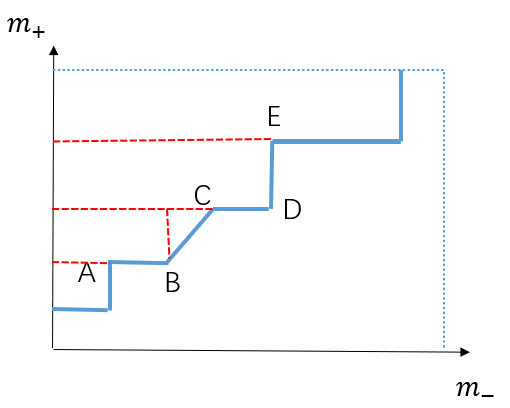
\includegraphics[scale=0.325]{2_5.png}
  % \caption{}
  \label{f4}
\end{figure}

令 $S_i$ 为ROC与y轴围成的面积块。则证明题目等式即证明 $\ell_{\mathrm{rank}}$ 是ROC曲线与轴围成的全部面积。

\begin{itemize}
  \item 平行于y轴的
\end{itemize}
此时,
$ \sum_{x^{+} \in D^{+}} \sum_{x^{-} \in D^{-}}\left( \frac{1}{2} \mathbb{I}\left(f\left(\boldsymbol{x}^{+}\right)=f\left(\boldsymbol{x}^{-}\right)\right) \right)= 0 $ ,\\
且$ \sum_{x^{+} \in D^{+}}\sum_{x^{-} \in D^{-}}\frac{1}{m^{+} m^{-}}\mathbb{I}\left(f\left(\boldsymbol{x}^{+}\right)<f\left(\boldsymbol{x}^{-}\right)\right) = \sum_{i,\text{平行y轴}} x_i n_i = \sum_{i,\text{平行y轴}} S_i $ ,\\
故,不妨令 $ \ell_{\mathrm{rank}} $ 前半部分求和是A,后半部分求和是B(方便打字),则:

$ \sum_{i,\text{平行y轴}} S_i  = A+B $ 得证;

\begin{itemize}
  \item 平行于x轴的
\end{itemize}
此时,$A+B=0$ ,$S=0$显然,因此,

$ \sum_{i,\text{平行x轴}}  S_i = A+B $ 得证;

\begin{itemize}
  \item 斜线段
\end{itemize}
此时,面积可以看成开始的点做y轴平行的线向上至结束的点的高度的与y轴围成的矩形加上斜线段与刚刚做的辅助线围成的三角形的面积之和。

其中, A为前者矩形的面积,B是三角形的面积,故

$ \sum_{i,\text{斜线段}} S_i  = A+B $ 得证.
\\

综上,$ \text{AUC} = 1-\ell_{\mathrm{rank}} $ 得证。



\subsection{}
$\chi^2 $ 检验过程:

对于我们要研究的指标,总体被分为 $k$ 类:$ A_i, i=1, 2, \dots, k $。理论上我们知道或者猜想这 $k$ 类数据占总体的比例为:

$H_0$ : $A_i$ 的占比为 $p_i, i = 1, 2, \dots, k$

检验这个原假设,根据收集的每个分类 $A_i$ 的实际频数 $n_i$ ,结合理论频数,有:
\begin{equation*}
  \sum_{i=1}^{k} \frac{\left(n_{i}-n p_{i}\right)^{2}}{n p_{i}} \sim \chi^{2}(k-1)
\end{equation*}
再通过查表比较大小,$\chi^{2}<\chi_{\alpha, k-1}^{2}$ 则没有充分理由拒绝原假设,认为实际符合理论。

(如果是连续数据则分段然后同上述离散的计算方式)





% ----------------section分割线-------------------------------------------

\section{HW3}
\begin{figure}[H]
  \centering
  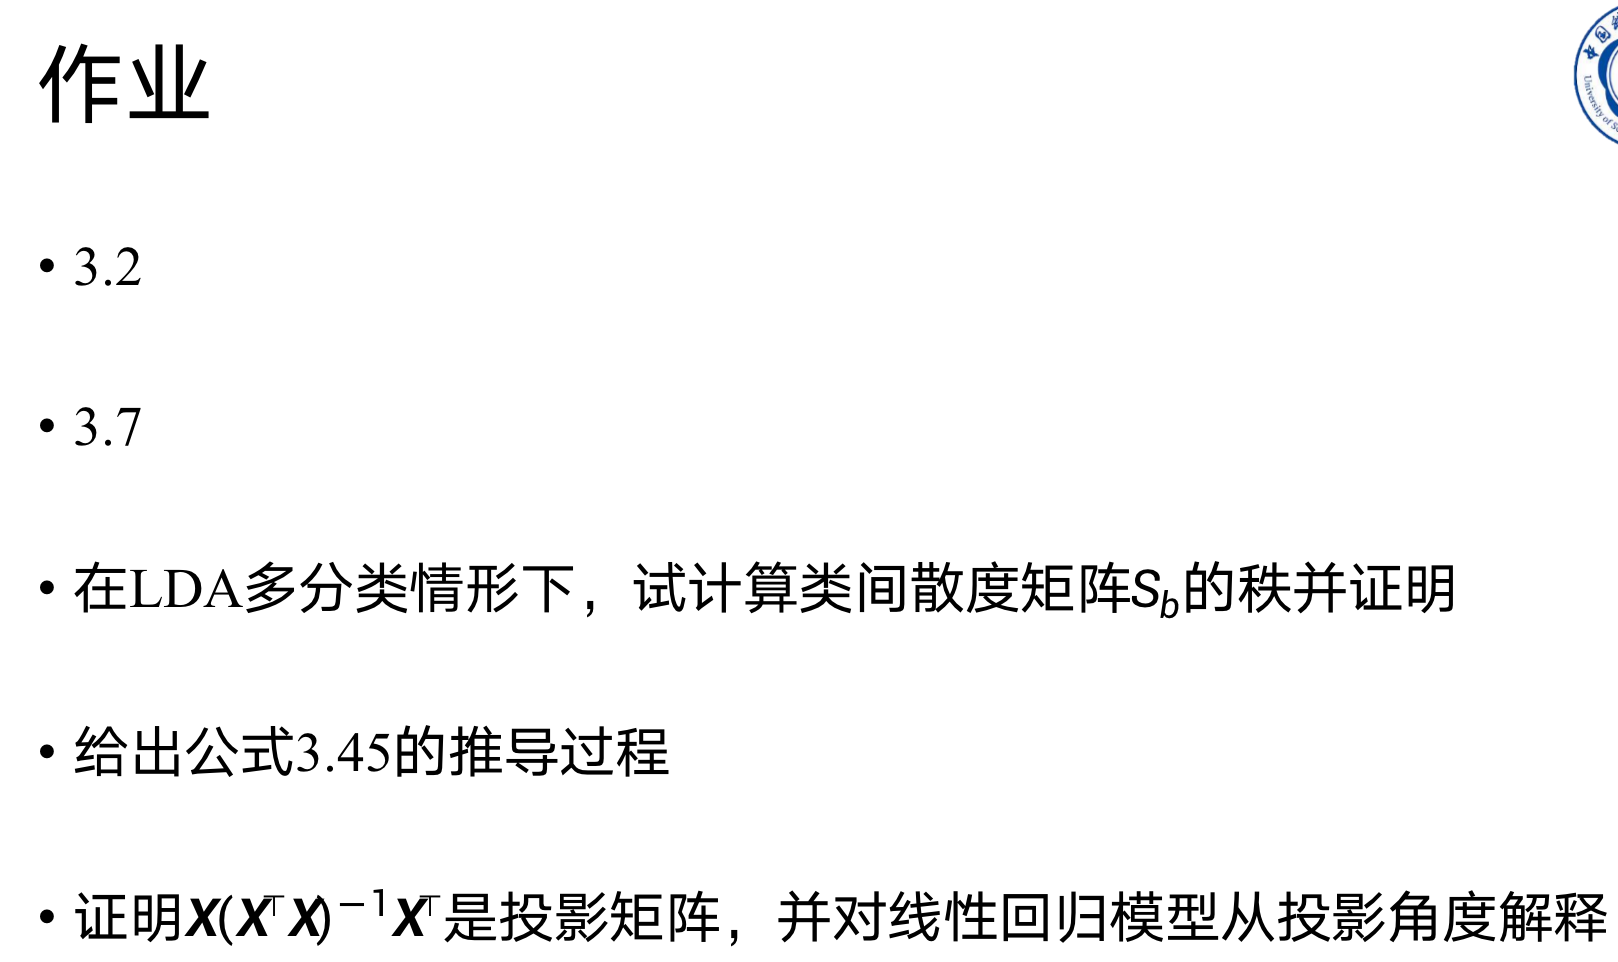
\includegraphics[scale=0.35]{hw3.png}
  % \caption{}
  \label{f5}
\end{figure}


\subsection{}

\begin{itemize}
  \item (3.18)
\end{itemize}

\begin{equation*}
  y=\frac{1}{1+e^{-\left(\boldsymbol{w}^{\mathrm{T}} \boldsymbol{x}+b\right)}}
\end{equation*}
一阶导数:
\begin{equation*}
  \frac{d y}{d w}=\frac{x e^{-\left(w^{T} x+b\right)}}{\left(1+e^{-\left(w^{T} x+b\right)}\right)^{2}}=x\left(y-y^{2}\right)
\end{equation*}
二阶导数:
\begin{equation*}
  \frac{d}{d w^{T}}\left(\frac{d y}{d w}\right)=x(1-2 y)\left(\frac{d y}{d w}\right)^{T}=x x^{T} y(y-1)(1-2 y)
\end{equation*}
对于 $ XPX^T $ ,有任意向量 $Z$ ,使得:
\begin{equation*}
  Z^{T} X P X^{T} Z=\sum_{i} P_{i i} V_{i}^{2} \geq 0
\end{equation*}
故,$ XPX^T $ 是半正定的。再由 $ y \in (0.5, 1) $ 时,$ y(y-1)(1-2 y) < 0 $ ,此时,(3.18) 的Hessian矩阵不是半正定的。
故,(3.18) 是非凸的。

\begin{itemize}
  \item (3.27)
\end{itemize}

\begin{equation*}
  \ell(\boldsymbol{\beta})=\sum_{i=1}^{m}\left(-y_{i} \boldsymbol{\beta}^{\mathrm{T}} \hat{\boldsymbol{x}}_{i}+\ln \left(1+e^{\boldsymbol{\beta}^{\mathrm{T}} \hat{\boldsymbol{x}}_{i}}\right)\right)
\end{equation*}
二阶导数:
\begin{equation*}
  \frac{d}{d \beta^{T}}\left(\frac{d l}{d \beta}\right)=x x^{T} p_1(x ; \beta)(1-p_1(x ; \beta))
\end{equation*}
其中,$p\in(0,1)$ ,故 $ p_1(x ; \beta)(1-p_1(x ; \beta) \geq 0 $ ,(3.27) 的Hessian矩阵是半正定的。
由此,(3.27) 是凸的。



\subsection{}

当 $3 \leq k \leq 7$ 时,需要长度 $2^{k-1}-1$ 的ECOC编码。在类别为4时,其可行的编码有7种,

% Table generated by Excel2LaTeX from sheet 'Sheet1'
\begin{table}[htbp]
  \centering
  % \caption{}
  \begin{tabular}{|l|ccccccl|}
    \toprule
       & f0 & f1 & f2 & f3 & f4 & f5 & f6 \\
    \midrule
    c1 & 1  & 1  & 1  & 1  & 1  & 1  & 1  \\
    c2 & 0  & 0  & 0  & 0  & 1  & 1  & 1  \\
    c3 & 0  & 0  & 1  & 1  & 0  & 0  & 1  \\
    c4 & 0  & 1  & 0  & 1  & 0  & 1  & 0  \\
    \bottomrule
  \end{tabular}%
  \label{tab:addlabel}%
\end{table}%
当码长为9时,那么之后加任意两个编码,即为最优编码,因为此时再加任意的编码都是先有编码的反码,此时,类别之间最小的海明距离都为4,不会再增加。



\subsection{}
在LDA多分类情形下, 试计算类间散度矩阵 $\mathrm{S}_{b}=\sum_{\mathrm{i}=1}^{\mathrm{N}} m_i\left(\mu_{\mathrm{i}}-\mu\right)\left(\mu_{\mathrm{i}}-\mu\right)^{\mathrm{T}}$ 的秩并证明.

\begin{equation*}
  \mathrm{S}_{b}= \left[\left(\mu_{1}-\mu\right),\left(\mu_{2}-\mu\right) \ldots\left(\mu_{N}-\mu\right)\right]\left(\begin{array}{lll}
      m_{1} &        &       \\
            & \ddots &       \\
            &        & m_{N}
    \end{array}\right)\left(\begin{array}{l}
      \left(\mu_{1}-\mu\right)^{T} \\
      \left(\mu_{2}-\mu\right)^{T} \\
      \vdots                       \\
      \left(\mu_{N}-\mu\right)^{T}
    \end{array}\right)
\end{equation*}
令 $M=\operatorname{diag}\left(m_{1}, m_{2}, \ldots, m_{N}\right), \mathrm{A}=\left(\mu_{1}-\mu, \mu_{2}-\mu, \ldots, \mu_{N}-\mu\right)^{T}$ ,则:
\begin{equation*}
  \begin{aligned}
    \operatorname{rank} (\mathrm{S}_{b}) & =\operatorname{rank} (A^{T} M A)                                                             \\
                                         & =\operatorname{rank} (A^{T} M^{\frac{1}{2}} M^{\frac{1}{2}} A)                               \\
                                         & =\operatorname{rank}\left(A^{T} M^{\frac{1}{2}}\right)\left(A^{T} M^{\frac{1}{2}}\right)^{T} \\
                                         & =\operatorname{rank}\left(A^{T} M^{\frac{1}{2}}\right)                                       \\
                                         & =\operatorname{rank} (A^{T})                                                                 \\
                                         & =\operatorname{rank}\left(\mu_{1}-\mu, \mu_{2}-\mu, \ldots, \mu_{N}-\mu\right)
  \end{aligned}
\end{equation*}
再由
\begin{equation*}
  \begin{aligned}
    \sum_{i=1}^{N} \boldsymbol{m}_{\boldsymbol{i}} \boldsymbol{\mu}_{\boldsymbol{i}}=\left(\sum_{i=1}^{N} \boldsymbol{m}_{\boldsymbol{i}}\right) \boldsymbol{\mu} \\
    \sum_{i=1}^{N} \boldsymbol{m}_{\boldsymbol{i}}\left(\boldsymbol{\mu}_{\boldsymbol{i}}-\boldsymbol{\mu}\right)=\mathbf{0}
  \end{aligned}
\end{equation*}
可知:$ \operatorname{rank} (\mathrm{S}_{b}) \leq N-1 $.



\subsection{}

由题得:

若$\boldsymbol{W}$ 为 (3.45) 的解。则对于任意常数与其的积也为解。不失一般性,令
$\operatornamewithlimits{tr}(\boldsymbol{W}^{\mathrm{T}} \mathbf{S}_{w} \boldsymbol{W})  = 1 $,则 (3.45) 等价为:
\begin{equation*}
  \begin{aligned}
    \min _{\boldsymbol{W}} & -\boldsymbol{W}^{\mathrm{T}} \mathbf{S}_{b} \boldsymbol{W}       \\
    \text { s.t. }         & \boldsymbol{W}^{\mathrm{T}} \mathbf{S}_{w} \boldsymbol{W}  = 1 .
  \end{aligned}
\end{equation*}
拉格朗日函数为:
\begin{equation*}
  L(\boldsymbol{W}, \lambda)=-\operatorname{tr}\left(\boldsymbol{W}^{\mathrm{T}} \boldsymbol{S}_{b} \boldsymbol{W}\right)+\lambda\left(\operatorname{tr}\left(\boldsymbol{W}^{\mathrm{T}} \boldsymbol{S}_{w} \boldsymbol{W}\right)-1\right)
\end{equation*}
于是有:
\begin{equation*}
  \begin{aligned}
    \mathrm{d} L & =-\operatorname{tr}\left((\mathrm{d} \boldsymbol{W})^{\mathrm{T}} \boldsymbol{S}_{b} \boldsymbol{W}+\boldsymbol{W}^{\mathrm{T}} \boldsymbol{S}_{b} \mathrm{~d} \boldsymbol{W}\right)+\lambda \operatorname{tr}\left((\mathrm{d} \boldsymbol{W})^{\mathrm{T}} \boldsymbol{S}_{w} \boldsymbol{W}+\boldsymbol{W}^{\mathrm{T}} \boldsymbol{S}_{w} \mathrm{~d} \boldsymbol{W}\right)                                                                                               \\
                 & =-\operatorname{tr}\left(\left(\boldsymbol{S}_{b} \boldsymbol{W}\right)^{\mathrm{T}} \mathrm{d} \boldsymbol{W}\right)-\operatorname{tr}\left(\boldsymbol{W}^{\mathrm{T}} \boldsymbol{S}_{b} \mathrm{~d} \boldsymbol{W}\right)+\lambda\left(\operatorname{tr}\left(\left(\boldsymbol{S}_{w} \boldsymbol{W}\right)^{\mathrm{T}} \mathrm{d} \boldsymbol{W}\right)+\operatorname{tr}\left(\boldsymbol{W}^{\mathrm{T}} \boldsymbol{S}_{w} \mathrm{~d} \boldsymbol{W}\right)\right) \\
                 & =\operatorname{tr}\left(\left[\lambda \boldsymbol{W}^{\mathrm{T}}\left(\boldsymbol{S}_{w}^{\mathrm{T}}+\boldsymbol{S}_{w}\right)-\boldsymbol{W}^{\mathrm{T}}\left(\boldsymbol{S}_{b}^{\mathrm{T}}+\boldsymbol{S}_{b}\right)\right] \mathrm{d} \boldsymbol{W}\right)                                                                                                                                                                                                           \\
                 & =\operatorname{tr}\left(\left[\left(\lambda\left(\boldsymbol{S}_{w}^{\mathrm{T}}+\boldsymbol{S}_{w}\right)-\left(\boldsymbol{S}_{b}^{\mathrm{T}}+\boldsymbol{S}_{b}\right)\right) \boldsymbol{W}\right]^{\mathrm{T}} \mathrm{d} \boldsymbol{W}\right)
  \end{aligned}
\end{equation*}
故可得到:
\begin{equation*}
  \frac{\partial L}{\partial W}=\left(\lambda\left(\boldsymbol{S}_{\mathrm{w}}^{\mathrm{T}}+\boldsymbol{S}_{w}\right)-\left(\boldsymbol{S}_{b}^{\mathrm{T}}+\boldsymbol{S}_{b}\right)\right) \boldsymbol{W}
\end{equation*}
偏导数为0时,有:
\begin{equation*}
  \boldsymbol{S}_{b} \boldsymbol{W}=\lambda \boldsymbol{S}_{w} \boldsymbol{W}
\end{equation*}

证毕.



\subsection{}
证明 $X(X^T X)^{-1} X^{T} $ 是投影矩阵, 并对线性回归模型从投影角度解释.

令 $P = X(X^T X)^{-1} X^{T}$ ,
\begin{equation*}
  \begin{aligned}
    P^2 & = (X(X^T X)^{-1} X^{T})(X(X^T X)^{-1} X^{T}) \\
        & = XI(X^T X)^{-1} X^{T}                       \\
        & = X(X^T X)^{-1} X^{T}                        \\
        & = P
  \end{aligned}
\end{equation*}
且,
\begin{equation*}
  P^T = (X(X^T X)^{-1} X^{T})^T = X(X^T X)^{-1} X^{T} = P
\end{equation*}

对X,
\begin{equation*}
  PX = X(X^T X)^{-1} X^{T}X = XI = X
\end{equation*}

故P是投影矩阵。

\begin{itemize}
  \item 解释
\end{itemize}
对于Ax = b来说,并不是任何时候都有解,实际上大多数这种类型的方程都无解。A的列空间的含义是方程组有解时b的取值空间,当b不在A的列空间时,方程无解。具体来说,当A是行数大于列数的长方矩阵时,方程组中的方程大于未知数个数,肯定无解。

虽然方程无解,这就需要转而寻找最接近可解问题的解。对于无解方程Ax = b,Ax总是在列空间里(因为列空间本来就是由Ax确定的,和b无关),
而b就不一定了,所以需要微调b,将b变成列空间中最接近它的一个,Ax = b变成了:
$A\hat{x}=p$

p就是A的列空间的投影, $\hat{x}$表示此时的x已经不是原来Ax = b中的x,$A\hat{x}\neq  b$,因为方程无解,所以不可能有Ax = b。
此时问题转换为寻找最好的A ,让它与原方程的差距最小:

假设A的秩是2,此时列空间的维度也是2,列空间将是一个平面,平面上的向量有无数个,其中最接近b的当然是b在平面上的投影,
只有b – p才能产生最小的误差向量.

所以说,想要求解不等方程Ax = b,需要将b微调成它在A的列空间上的投影(列空间上的向量很多,b在列空间上的投影是唯一的)。
如果b在列空间中,b的投影就是它自己;如果b正交于列空间,它的投影是0。





% ----------------section分割线-------------------------------------------

\section{HW4}

\begin{figure}[H]
  \centering
  \begin{minipage}[t]{0.48\textwidth}
    \centering
    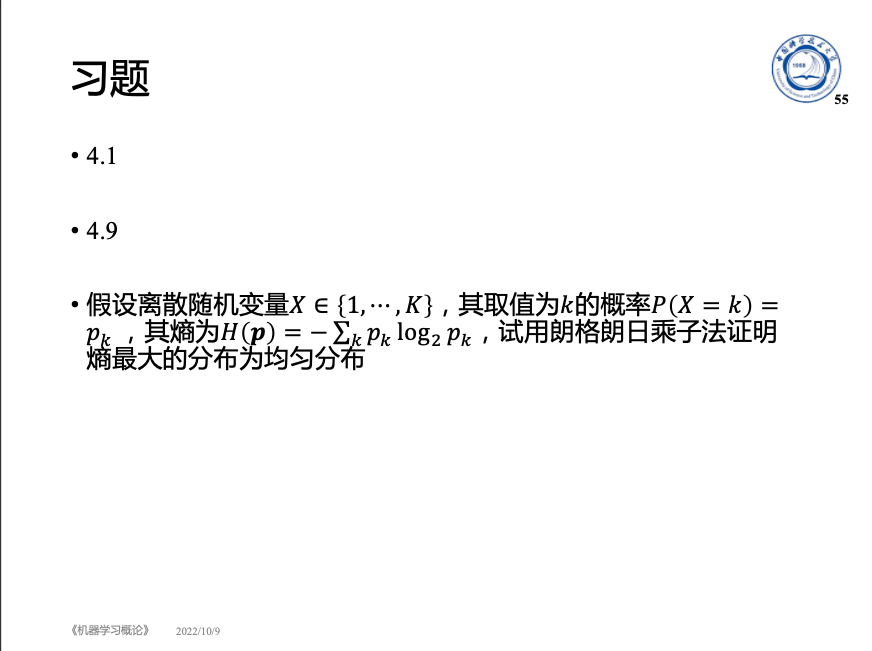
\includegraphics[width=6.5cm]{hw4.1.png}
    % \caption{}
  \end{minipage}
  \begin{minipage}[t]{0.48\textwidth}
    \centering
    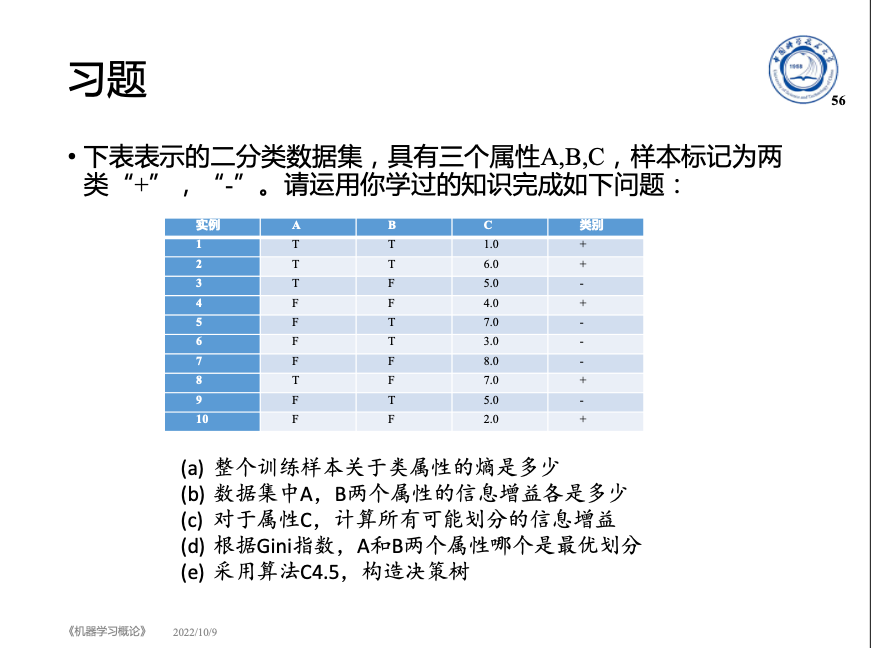
\includegraphics[width=6.5cm]{hw4.2.png}
    % \caption{}
  \end{minipage}
\end{figure}



\subsection{}

因为决策树是通过属性来划分,相同属性的样本最终肯定会进入相同的叶节点。一个叶节点只有一个分类,如果样本属性相同而分类不同,必然产生训练误差。反之,决策树只会在当前样本集合是同一类或者所有属性相同时才会停止划分,最终得到训练误差为0的决策树。



\subsection{}

数据集$D$的纯度Gini:
\begin{equation*}
  \operatorname{Gini}(D)=1-\sum_{k=1}^{|y|}{{p_{k}}}^{2} = \sum_{k=1}^{|y|}{{p_{k}}}(1-p_k)
\end{equation*}
属性$a$ 的纯度Gini-index:
\begin{equation*}
  \operatorname{Gini}_{-} index(D,a) = \sum_{v=1}^{v} \frac{\left|D^{v}\right|}{|D|} \operatorname{Gini}\left(D^{v}\right)
\end{equation*}
记$\tilde{D}$ 为$D$中在属性$a$上没有缺失值的样本子集,$\tilde{D}^v$为$\tilde{D}$在属性$a$上取值为$a^v$的样本子集。
属性  $a$  的基尼指数可推广为:
\begin{equation*}
  \operatorname{Gini}_{-} index  (D, a)=p \times \operatorname{Gini}_{-} index(\tilde{D}, a)=p \times \sum_{v=1}^{V} \tilde{v} G i n i\left(D^{v}\right)
\end{equation*}



\subsection{}

拉格朗日函数为:
\begin{equation*}
  L(\boldsymbol{p}, \lambda)=-\sum_{i=1}^{K} p_{i} \log _{2} p_{i}+\lambda\left(\sum_{i=1}^{K} p_{i}-1\right)
\end{equation*}
则:
\begin{equation*}
  \frac{\partial L(p, \lambda)}{\partial p_{i}}=-\log _{2} p_{i}-\frac{1}{\ln 2}+\lambda=0
\end{equation*}
\begin{equation*}
  \frac{\partial L(p, \lambda)}{\partial \lambda}=\sum_{i=1}^{K} p_{i}-1=0
\end{equation*}
且$ p_1=p_2=\dots=p_k=2^{\lambda-\frac{1}{\ln 2}} $,
由$ \sum_{i=1}^Kp_i=1 $得:
\begin{equation*}
  p_1=p_2=\dots=p_k=\frac{1}{K}
\end{equation*}

拉朗格由上述方程组解出$p_i$及$\lambda$ ,如此求得的$p_i$,就是函数$L(\boldsymbol{p}, \lambda)$在附加条件
$ \sum_{i=1}^Kp_i=1 $下的可能的极值点。若这样的点只有一个,由实际问题可直接确定此即所求的点,因此熵的最大分布为均匀分布。



\subsection{}

\subsubsection{}
10个样本中,正例5个,负例5个,故:
\begin{equation*}
  \operatorname{Ent}(D) = -(0.5\log_2 0.5)\times2 = 1
\end{equation*}

\subsubsection{}
A中 'T' 4个(里面正例3个),'F' 6个(里面正例2个);B中 'T' 5个(里面正例2个),'F' 5个(里面正例3个),故:
\begin{equation*}
  \begin{aligned}
    \operatorname{Gain}(D,A) & = \operatorname{Ent}(D)-\sum_{v=1}^{V} \frac{\left|D^{v}\right|}{|D|} \operatorname{Ent}\left(D^{v}\right)                   \\
                             & = 1 + 0.4\times(0.75\log_2 0.75 + 0.25\log_2 0.25) + 0.6\times(\frac{2}{6}\log_2 \frac{2}{6} + \frac{4}{6}\log_2\frac{4}{6}) \\
                             & = 0.1245
  \end{aligned}
\end{equation*}
\begin{equation*}
  \begin{aligned}
    \operatorname{Gain}(D,B) & = \operatorname{Ent}(D)-\sum_{v=1}^{V} \frac{\left|D^{v}\right|}{|D|} \operatorname{Ent}\left(D^{v}\right) \\
                             & = 1 + 0.5\times(0.6\log_2 0.6 + 0.4\log_2 0.4) + 0.5\times(0.6\log_2 0.6 + 0.4\log_2 0.4)                  \\
                             & = 0.0290
  \end{aligned}
\end{equation*}

\subsubsection{}
属性C有8个取值1,2,3,4,5,6,7,8. 其中5(2负)和7(一正一负)有两个样本其余一个。7种二分阈值的信息增益分别为:
% \begin{equation*}
%   \begin{aligned}
%     \operatorname{Gain}(D,C) &= \operatorname{Ent}(D)-\sum_{v=1}^{V} \frac{\left|D^{v}\right|}{|D|} \operatorname{Ent}\left(D^{v}\right)\\
%     &= 1 - 6\times\frac{1}{10}\times 0 - \frac{2}{10}\times 0 - \frac{2}{10}\times 1\\
%     &= 0.8
%   \end{aligned}
% \end{equation*}
\begin{enumerate}
  \item 1, 2-8:
        \begin{equation*}
          \begin{aligned}
            \operatorname{Gain}(D,C) & = \operatorname{Ent}(D)-\sum_{v=1}^{V} \frac{\left|D^{v}\right|}{|D|} \operatorname{Ent}\left(D^{v}\right) \\
                                     & = 1 - \frac{1}{10}\times 0 - \frac{9}{10}\times 0.9911                                                     \\
                                     & = 0.1080
          \end{aligned}
        \end{equation*}
  \item 1-2, 3-8:
        \begin{equation*}
          \begin{aligned}
            \operatorname{Gain}(D,C) & = \operatorname{Ent}(D)-\sum_{v=1}^{V} \frac{\left|D^{v}\right|}{|D|} \operatorname{Ent}\left(D^{v}\right) \\
                                     & = 1 - \frac{2}{10}\times 0 - \frac{8}{10}\times 0.9544                                                     \\
                                     & = 0.2364
          \end{aligned}
        \end{equation*}
  \item 1-3, 4-8:
        \begin{equation*}
          \begin{aligned}
            \operatorname{Gain}(D,C) & = \operatorname{Ent}(D)-\sum_{v=1}^{V} \frac{\left|D^{v}\right|}{|D|} \operatorname{Ent}\left(D^{v}\right) \\
                                     & = 1 - \frac{3}{10}\times 0.9183 - \frac{7}{10}\times 0.9852                                                \\
                                     & = 0.0349
          \end{aligned}
        \end{equation*}
  \item 1-4, 5-8:
        \begin{equation*}
          \begin{aligned}
            \operatorname{Gain}(D,C) & = \operatorname{Ent}(D)-\sum_{v=1}^{V} \frac{\left|D^{v}\right|}{|D|} \operatorname{Ent}\left(D^{v}\right) \\
                                     & = 1 - \frac{4}{10}\times 0.8113 - \frac{6}{10}\times 0.9183                                                \\
                                     & = 0.1245
          \end{aligned}
        \end{equation*}
  \item 1-5, 6-8:
        \begin{equation*}
          \begin{aligned}
            \operatorname{Gain}(D,C) & = \operatorname{Ent}(D)-\sum_{v=1}^{V} \frac{\left|D^{v}\right|}{|D|} \operatorname{Ent}\left(D^{v}\right) \\
                                     & = 1 - \frac{6}{10}\times 1 - \frac{4}{10}\times 1                                                          \\
                                     & = 0
          \end{aligned}
        \end{equation*}
  \item 1-6, 7-8:
        \begin{equation*}
          \begin{aligned}
            \operatorname{Gain}(D,C) & = \operatorname{Ent}(D)-\sum_{v=1}^{V} \frac{\left|D^{v}\right|}{|D|} \operatorname{Ent}\left(D^{v}\right) \\
                                     & = 1 - \frac{7}{10}\times 0.9852 - \frac{3}{10}\times 0.9183                                                \\
                                     & = 0.0148
          \end{aligned}
        \end{equation*}
  \item 1-7, 8:
        \begin{equation*}
          \begin{aligned}
            \operatorname{Gain}(D,C) & = \operatorname{Ent}(D)-\sum_{v=1}^{V} \frac{\left|D^{v}\right|}{|D|} \operatorname{Ent}\left(D^{v}\right) \\
                                     & = 1 - \frac{9}{10}\times 0.9911 - \frac{1}{10}\times 0                                                     \\
                                     & = 0.1080
          \end{aligned}
        \end{equation*}
\end{enumerate}



\subsubsection{}
由基尼值的定义:
\begin{equation*}
  \begin{aligned}
    \operatorname{Gini}(D) & =\sum_{k=1}^{|\mathcal{Y}|} \sum_{k^{\prime} \neq k} p_{k} p_{k^{\prime}} \\
                           & =1-\sum_{k=1}^{|\mathcal{Y}|} p_{k}^{2}
  \end{aligned}
\end{equation*}

对于A,B的Gini指数:
\begin{equation*}
  \begin{aligned}
    \operatorname{Gini} \text { index }(D, A) & =\sum_{v=1}^{V} \frac{\left|D^{v}\right|}{|D|} \operatorname{Gini}\left(D^{v}\right) \\
                                              & = 0.4\times (1-0.75^2-0.25^2) + 0.6\times (1-(\frac{2}{6})^2-(\frac{4}{6})^2)        \\
                                              & = 0.4167
  \end{aligned}
\end{equation*}
\begin{equation*}
  \begin{aligned}
    \operatorname{Gini} \text { index }(D, B) & =\sum_{v=1}^{V} \frac{\left|D^{v}\right|}{|D|} \operatorname{Gini}\left(D^{v}\right) \\
                                              & = 0.5\times (1-0.4^2-0.6^2) \times 2                                                 \\
                                              & = 0.48
  \end{aligned}
\end{equation*}

所以A的Gini指数小,划分最优。

\subsubsection{}
由前几小题可知:
C的信息增益选择第2种划分方式增益最大,由此选第二种作为C的处理方式。此时,

\begin{equation*}
  \begin{aligned}
     & \operatorname{GainRatio}(D,A) = \frac{\operatorname{Gain}(D,A)}{\operatorname{IV}(A)} = \frac{0.1245}{0.9710} = 0.1232 \\
     & \operatorname{GainRatio}(D,B) = \frac{\operatorname{Gain}(D,B)}{\operatorname{IV}(B)} = \frac{0.0290}{1} = 0.0290      \\
     & \operatorname{GainRatio}(D,C) = \frac{\operatorname{Gain}(D,C)}{\operatorname{IV}(C)} = \frac{0.2364}{0.7219} = 0.3275
  \end{aligned}
\end{equation*}

所以第一层选择C。此时,
对于C的1-2子树全为正例,没必要继续计算,该子树直接判断为正例;对于3-7子树有:

\begin{equation*}
  \begin{aligned}
     & \operatorname{GainRatio}(D',A) = \frac{\operatorname{Gain}(D',A)}{\operatorname{IV}'(A)} = \frac{0.9544-0.9512}{0.9544} = 0.003388 \\
     & \operatorname{GainRatio}(D',B) = \frac{\operatorname{Gain}(D',B)}{\operatorname{IV}'(B)} = \frac{0.9544-0.9056}{1} = 0.04876
  \end{aligned}
\end{equation*}

所以该子树选择B作为第二层。对于第三层,由表格数据可知:B的‘T’类:A为‘T’则判断为正类,A为‘F’则判断为负类;
B的‘F’类:A为‘T’由于正负都各出现一次,因此都可以,A为‘F’则判断为正类。





% ----------------section分割线-------------------------------------------

\section{HW5}

\begin{figure}[H]
  \centering
  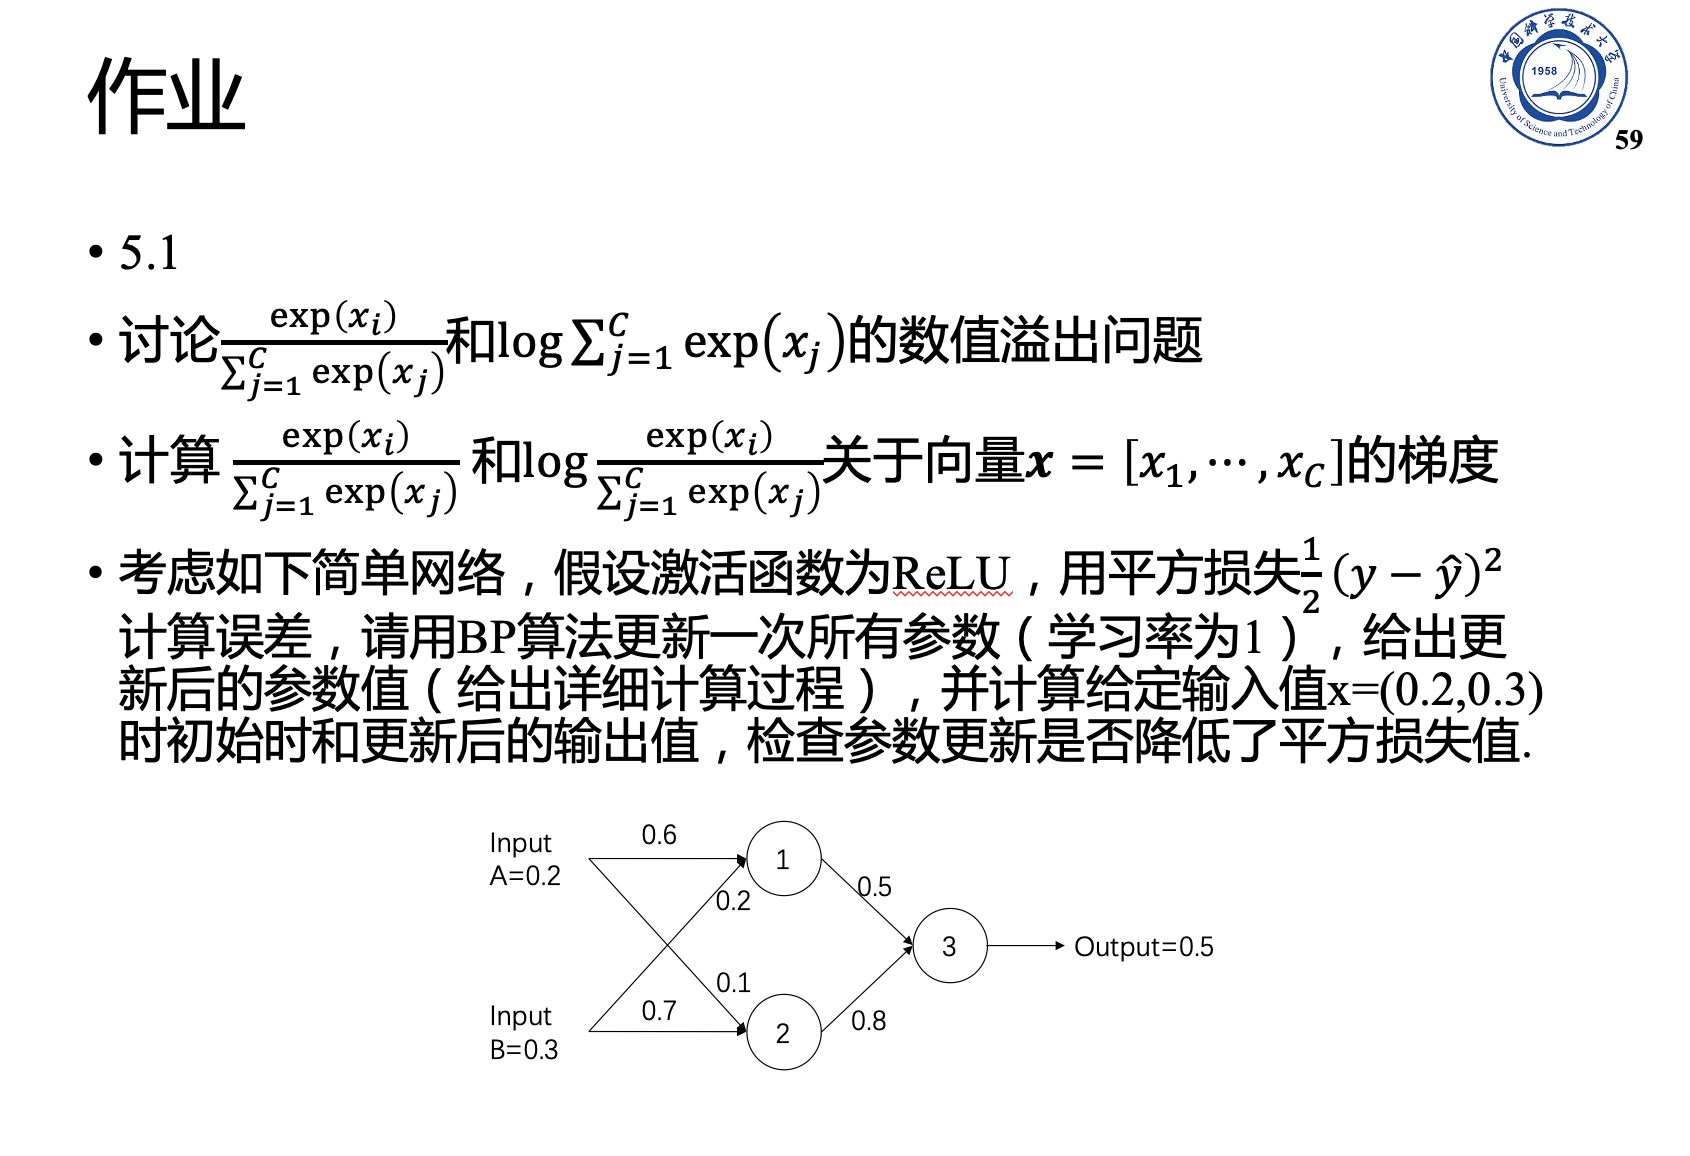
\includegraphics[scale=0.35]{hw5.png}
  % \caption{}
  \label{f6}
\end{figure}


\subsection{}

理想中的激活函数是阶跃函数,但是阶跃函数非连续,在0处不可导;线性激活函数没办法完全的拟合阶跃函数。
线性函数在定义域内变换情况相同。
使用线性函数作为激活函数时,无论是在隐藏层还是在输出层,不管传递多少层,
其单元值都还是输入值和 $x$ 的线性组合,若输出层也使用线性函数作为激活函数,
那么就等价于线性回归,达不到激活与筛选的目的。



\subsection{}

\begin{itemize}
  \item $ \frac{e^{x_i}}{\sum_{j=1}^n e^{x_j}} $
\end{itemize}
如果$x_i$很大,那么指数操作时可能会大于数据类型容许的最大数字,造成上溢,这将使分母或分子变为$\infty$,
这就使得结果是$0, \infty$还是 nan难以得到准确结论。
但可以在计算之前对所有的$x_i$减去max($x_i$)避免上溢。
% (这时可能会可能存在一些具有较大负值造成下溢)。
\begin{itemize}
  \item $ \log{\sum_{j=1}^n e^{x_j}} $
\end{itemize}
一样的原因,$e^{x_i}$计算可能溢出,也可以做同样处理,取c=max($x_i$),
\begin{equation*}
  \begin{aligned}
    \log \left(\sum_{\mathrm{i}=1}^{\mathrm{n}} \mathrm{e}^{\mathrm{x}_{\mathrm{i}}}\right)
     & =\log \left(\sum_{\mathrm{i}=1}^{\mathrm{n}} \mathrm{e}^{\mathrm{x}_{\mathrm{i}}-\mathrm{c}} \mathrm{e}^{\mathrm{c}}\right)                   \\
     & =\log \left(\mathrm{e}^{\mathrm{c}} \sum_{\mathrm{i}=1}^{\mathrm{n}} \mathrm{e}^{\mathrm{x}_{\mathrm{i}}-\mathrm{c}}\right)                   \\
     & =\log \left(\sum_{\mathrm{i}=1}^{\mathrm{n}} \mathrm{e}^{\mathrm{x}_{\mathrm{i}}-\mathrm{c}}\right)+\log \left(\mathrm{e}^{\mathrm{c}}\right) \\
     & =\log \left(\sum_{\mathrm{i}=1}^{\mathrm{n}} \mathrm{e}^{\mathrm{x}_{\mathrm{i}}-\mathrm{c}}\right)+\mathrm{c}
  \end{aligned}
\end{equation*}



\subsection{}

记$ f(x) = \frac{e^{x_i}}{\sum_{j=1}^C e^{x_j}} $
\begin{equation*}
  \frac{\partial f(x)}{\partial x_{k}}=\left\{\begin{array}{ll}
    -\frac{\exp \left(x_{i}+x_{k}\right)}{\sum_{j=1}^{C} \exp \left(x_{j}\right)^{2}},                                           & k \neq i \\
    \frac{\exp \left(x_{k}\right) \sum_{j=1, j \neq k}^{C} \exp \left(x_{j}\right)}{\sum_{j=1}^{C} \exp \left(x_{j}\right)^{2}}, & k=i
  \end{array}\right.
\end{equation*}

记$ g(x) = \log \frac{e^{x_i}}{\sum_{j=1}^C e^{x_j}} $
\begin{equation*}
  \frac{\partial g(x)}{\partial x_{k}}=\left\{\begin{array}{ll}
    -\frac{\exp \left(x_{k}\right)}{\sum_{j=1}^{C} \exp \left(x_{j}\right)},  & k \neq i \\
    1-\frac{\exp \left(x_{k}\right)}{\sum_{j=1}^{C} \exp \left(x_{j}\right)}, & k=i
  \end{array}\right.
\end{equation*}



\subsection{}

由题得:
\begin{equation*}
  \begin{aligned}
     & h_1 = 0.6\times 0.2 + 0.2\times 0.3 = 0.18 \\
     & h_2 = 0.1\times 0.2 + 0.7\times 0.3 = 0.23
  \end{aligned}
\end{equation*}
经过激活函数ReLU: max(0,x)变换后值为:
\begin{equation*}
  \begin{aligned}
     & out_{h_1} = max(0,h_1) = 0.18 \\
     & out_{h_2} = max(0,h_2) = 0.23
  \end{aligned}
\end{equation*}
所以输出值:
\begin{equation*}
  Output = 0.18\times 0.5 + 0.23\times 0.8 = 0.274
\end{equation*}
此时误差为:
\begin{equation*}
  E = \frac{1}{2} (0.5-0.274)^2 = 0.025538
\end{equation*}

BP(标准):
记$out_{h_1}: o_1$, $out_{h_2}: o_2$
由于:
\begin{equation*}
  E = \frac{1}{2} (y - w_5 o_1 -w_6 o_2 )^2
\end{equation*}
故可得到:
\begin{equation*}
  \frac{\partial E}{\partial w_5} = -o_1(y - w_5 o_1 -w_6 o_2 )
\end{equation*}
一次更新:
\begin{equation*}
  \begin{aligned}
    w_{5new} & = w_{5old} - \eta \frac{\partial E}{\partial w_{5old}} \\
             & = 0.5 - 1\times (-0.18(0.5-0.274))                     \\
             & = 0.54068
  \end{aligned}
\end{equation*}
同理:
\begin{equation*}
  \begin{aligned}
    w_{6new} & = w_{6old} - \eta \frac{\partial E}{\partial w_{6old}} \\
             & = 0.8 - 1\times (-0.23(0.5-0.274))                     \\
             & = 0.85198
  \end{aligned}
\end{equation*}
此时有:$h_1=o_1,h_2=o_2$,故由于:
\begin{equation*}
  h_1 = w_1A+w_3B
\end{equation*}
有:
\begin{equation*}
  \begin{aligned}
    E & = \frac{1}{2} (y - w_5 o_1 -w_6 o_2 )^2         \\
      & = \frac{1}{2} (y - w_5 h_1 -w_6 h_2 )^2         \\
      & = \frac{1}{2} (y - w_5 (w_1A+w_3B) -w_6 h_2 )^2
  \end{aligned}
\end{equation*}
\begin{equation*}
  \frac{\partial E}{\partial w_1} = -w_5A(y - w_5 (w_1A+w_3B) -w_6 h_2)
\end{equation*}
所以:
\begin{equation*}
  \begin{aligned}
    w_{1new} & = w_{1old} - \eta\frac{\partial E}{\partial w_{1old}} \\
             & = 0.6 - 1\times (-0.5\times 0.2(0.5 - 0.274))         \\
             & = 0.6226
  \end{aligned}
\end{equation*}
同理:
\begin{equation*}
  \begin{aligned}
    w_{3new} & = w_{3old} - \eta\frac{\partial E}{\partial w_{3old}} \\
             & = 0.2 - 1\times (-0.5\times 0.3(0.5 - 0.274))         \\
             & = 0.2339
  \end{aligned}
\end{equation*}
\begin{equation*}
  \begin{aligned}
    w_{2new} & = w_{2old} - \eta\frac{\partial E}{\partial w_{2old}} \\
             & = 0.1 - 1\times (-0.8\times 0.2(0.5 - 0.274))         \\
             & = 0.13616
  \end{aligned}
\end{equation*}
\begin{equation*}
  \begin{aligned}
    w_{4new} & = w_{4old} - \eta\frac{\partial E}{\partial w_{4old}} \\
             & = 0.7 - 1\times (-0.8\times 0.3(0.5 - 0.274))         \\
             & = 0.75424
  \end{aligned}
\end{equation*}
此时,更新后的输出值为:
\begin{equation*}
  \begin{aligned}
    Output_{new} & = max((0.6226\times 0.2 + 0.2339\times 0.3),0)\times 0.54068 \\&+ max((0.13616\times 0.2 + 0.75424\times 0.3),0)\times 0.85198\\
                 & = 0.32125
  \end{aligned}
\end{equation*}
平方损失:
\begin{equation*}
  E_{new} = \frac{1}{2} (0.5-0.32125)^2 = 0.01598 < 0.025538
\end{equation*}
因此参数更新降低了平方损失值。





% ----------------section分割线-------------------------------------------

\section{HW6}

\begin{figure}[H]
  \centering
  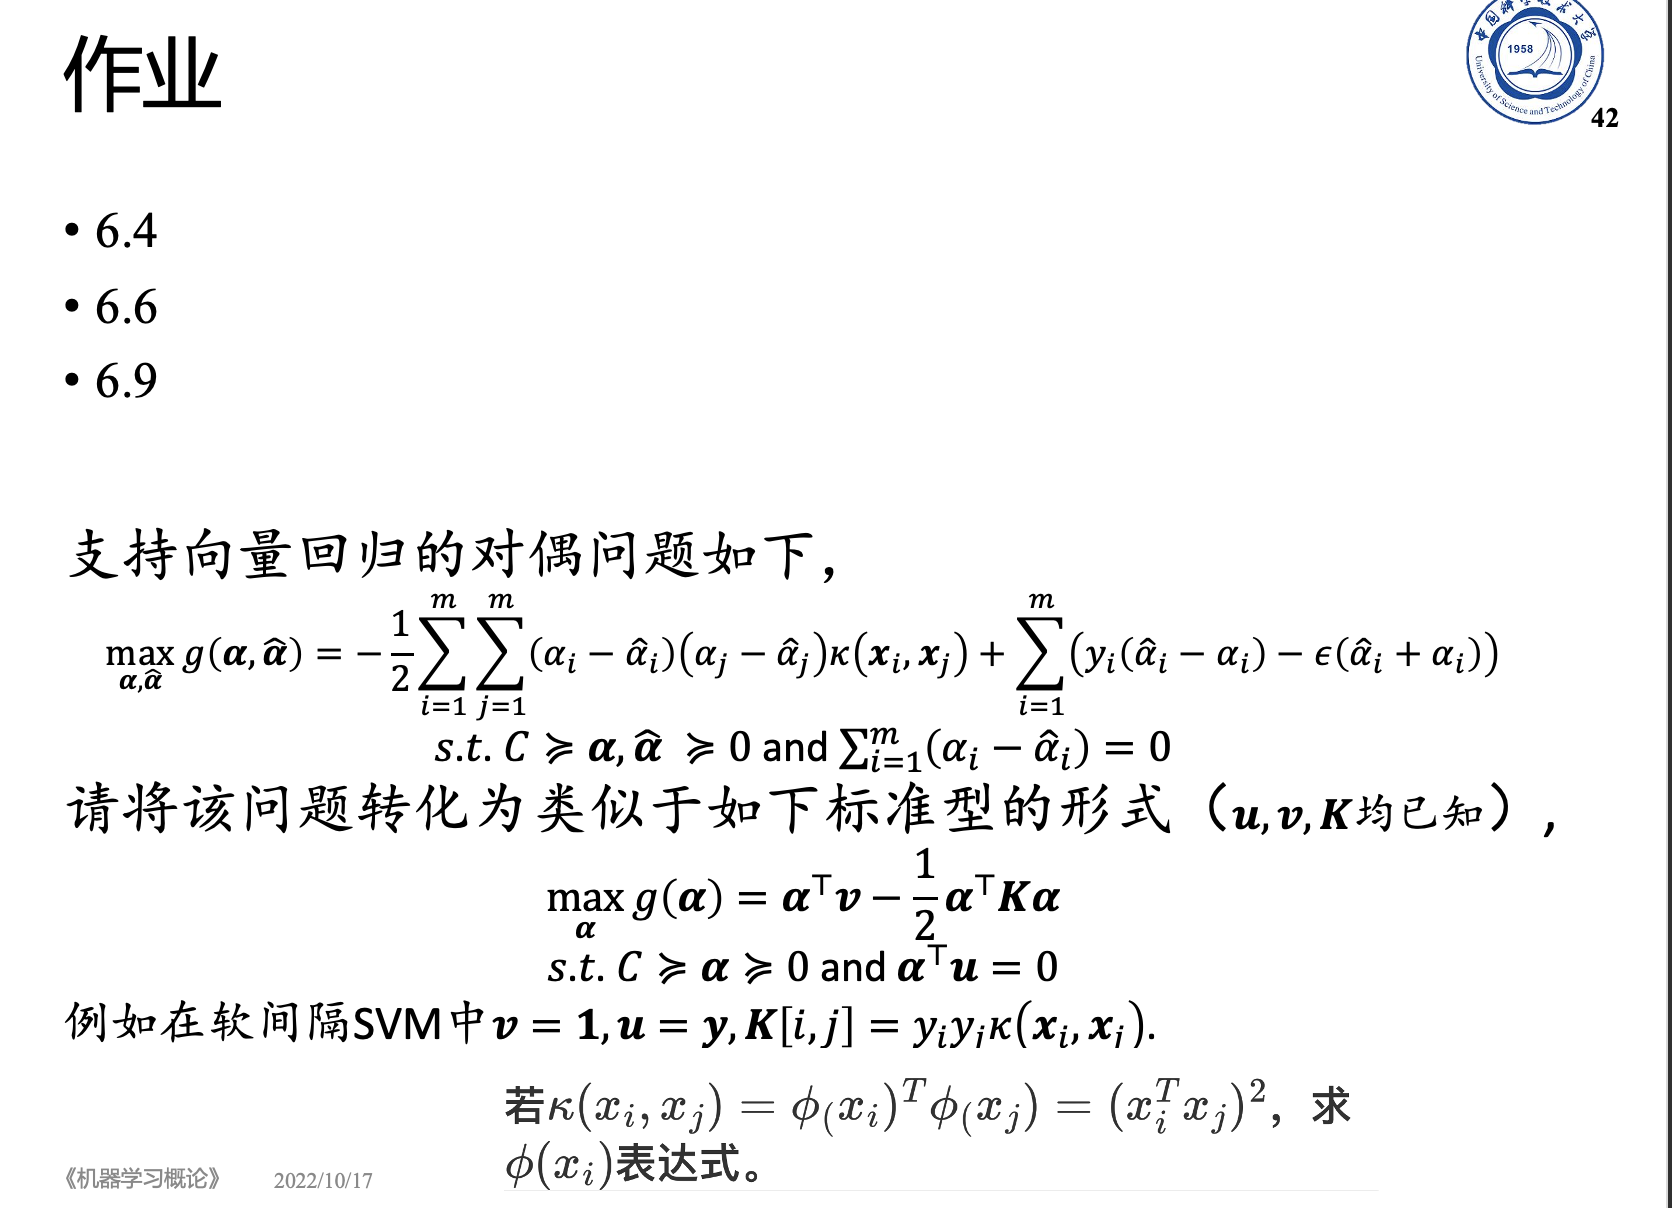
\includegraphics[scale=0.35]{hw6.png}
  % \caption{}
  \label{f7}
\end{figure}


\subsection{}

线性判别分析能够解决多分类问题, 而SVM只能解决二分类问题。
故当两类样本线性可分时,且处理二分类问题时等价。



\subsection{}

SVM的目的是求出与支持向量有最大化距离的直线,以每个样本为圆心,该距离为半径做圆,
可以近似认为圆内的点与该样本属于相同分类。
如果出现了噪声,那么这个噪声所带来的错误分类也将最大化,所以SVM对噪声是很敏感的。



\subsection{}

使用对率损失函数 $\ell_{log}$ 来代替式 (6.29) 中的 0/1损失函数,则几乎就得到了对率回归模型 (3.27),即:\\
由SVM模型:
\begin{equation*}
  \min _{\boldsymbol{w}, b} \frac{1}{2}\|\boldsymbol{w}\|^{2} \quad \text { s.t. } y_{i}\left(\boldsymbol{w}^{\top} \boldsymbol{x}_{i}+b\right) \geq 1 \quad i=1, \cdots, m
\end{equation*}
软间隔的支持向量机:
\begin{equation*}
  \min _{\boldsymbol{w}, b} \frac{1}{2}\|\boldsymbol{w}\|^{2}+C \sum_{i=1}^{m} \ell_{0 / 1}\left(y_{i}\left(\boldsymbol{w}^{\top} \phi\left(\boldsymbol{x}_{i}\right)+b\right)-1\right)
\end{equation*}
令$y_{i}\left(\boldsymbol{w}^{\top} \phi\left(\boldsymbol{x}_{i}\right)+b\right)=Z$,对率损失:
\begin{equation*}
  \ell_{\log }(z)=\log \left(1+e^{-z}\right)=\log \left(\frac{1+e^{z}}{e^{z}}\right)=\log \left(1+e^{z}\right)-z
\end{equation*}
即核对率回归:
\begin{equation*}
  \min _{w, b} \frac{1}{2}\|w\|^{2}+C \sum_{i=1}^{m}\left(-z+\log \left(1+e^{z}\right)\right)
\end{equation*}
\begin{equation*}
  \ell(\beta)=\sum_{i=1}^{m}\left(-y_{i} \beta^{\top} \widehat{x}_{i}+\log \left(1+e^{\beta^{\top} \widehat{x}_{i}}\right)\right)
\end{equation*}



\subsection{}

令
\begin{equation*}
  \begin{array}{c}
    \boldsymbol{\alpha}=\left(\begin{array}{c}
        \alpha \\
        \hat{\alpha}
      \end{array}\right) \in \mathbb{R}^{2 m}, v=\left(\begin{array}{c}
        -\boldsymbol{y}-\epsilon \\
        \boldsymbol{y}-\epsilon
      \end{array}\right) \in \mathbb{R}^{2 m} \\
    \boldsymbol{K}=\left(\begin{array}{cc}
        K  & -K \\
        -K & K
      \end{array}\right) \in \mathbb{R}^{2 m \times 2 m} \text { 其中 } K_{i j}=\boldsymbol{\kappa}\left(\boldsymbol{x}_{i}, \boldsymbol{x}_{j}\right)
  \end{array}
\end{equation*}
则可以得到结论.

\begin{equation*}
  \begin{aligned}
    \kappa\left(x_{i}, x_{j}\right) & =\left(x_{i}^{T} x_{j}\right)^{2}                                                        \\
                                    & =\left(x_{i}^{T} x_{j}\right)\left(x_{i}^{T} x_{j}\right)                                \\
                                    & =\left(\sum_{p=1}^{d} x_{p i} x_{p j}\right)\left(\sum_{q=1}^{d} x_{q i} x_{q j}\right)  \\
                                    & =\sum_{p=1}^{d} \sum_{q=1}^{d} x_{p i} x_{p j} x_{q i} x_{q j}                           \\
                                    & =\left(\begin{array}{c}
        x_{1} x_{1} \\
        x_{1} x_{2} \\
        \vdots      \\
        x_{1} x_{d} \\
        \vdots      \\
        x_{2} x_{d} \\
        \vdots      \\
        x_{d} x_{1} \\
        \vdots      \\
        x_{d} x_{d}
      \end{array}\right) \times\left(\begin{array}{c}
        x_{1} x_{1} \\
        x_{1} x_{2} \\
        \vdots      \\
        x_{1} x_{d} \\
        \vdots      \\
        x_{2} x_{d} \\
        \vdots      \\
        x_{d} x_{1} \\
        \vdots      \\
        x_{d} x_{d}
      \end{array}\right)
  \end{aligned}
\end{equation*}
则可以得到:
\begin{equation*}
  \phi: \boldsymbol{x} \in \mathbb{R}^{d} \rightarrow\left(\begin{array}{c}
      x_{1} x_{1} \\
      x_{1} x_{2} \\
      \vdots      \\
      x_{1} x_{d} \\
      \vdots      \\
      x_{2} x_{d} \\
      \vdots      \\
      x_{d} x_{1} \\
      \vdots      \\
      x_{d} x_{d}
    \end{array}\right) \in \mathbb{R}^{d^{2}}
\end{equation*}





% ----------------section分割线-------------------------------------------

\section{HW7}

\begin{figure}[H]
  \centering
  
\includegraphics[scale=0.675]{hw7.png}
  % \caption{}
  \label{f:hw7}
\end{figure}


\subsection{}

\begin{quotation}
  实践中使用式(7.15)决定分类类别时,若数据的维数非常高,则概率连
  乘 $ \prod_{i=1}^{d} P(x_i|c)  $ 的结果通常会非常接近于0 从而导致下溢.
  试述防止下溢的可能方案.
\end{quotation}

(7.15):
\begin{equation*}
  h_{n b}(\boldsymbol{x})=\underset{c \in \mathcal{Y}}{\arg \max } P(c) \prod_{i=1}^{d} P\left(x_{i} \mid c\right)
\end{equation*}

若连乘的式子太多,导致乘积接近0。由于属性个数是已知的,可以对每个乘式做适当次的开方处理,
可以保证结果不会为0。
另外也可以对各项取对数,当累加太多时,可能导致和接近负无穷。
可以对每个加数除以属性的个数,来防止溢出。



\subsection{}

\begin{quotation}
  试证明:二分类任务中两类数据满足高斯分布且方差相同时,线性判
  别分析产生贝叶斯最优分类器.
\end{quotation}

假设1类样本均值为 $u_1$, 2类样本均值为 $u_2$.

由题意,数据满足高斯分布且方差相同,因此,当样本足够大时,认为等价于:
线性判别分析公式
$ J=\frac{\left|w^{T}\left(u_{1}-u_{2}\right)\right|^{2}}{w^{T}\left(\Sigma_{1}+\Sigma_{2}\right) w} $
求最大值;对
$ \frac{1}{J}=\frac{w^{T}\left(\Sigma_{1}+\Sigma_{2}\right) w}{\left|w^{T}\left(u_{1}-u_{2}\right)\right|^{2}}=\sum_{i} \frac{\left(1-y_{i}\right)\left|w^{T}\left(x_{i}-u_{1}\right)\right|^{2}+y_{i}\left|w^{T}\left(x_{i}-u_{2}\right)\right|^{2}}{\left|w^{T}\left(u_{1}-u_{2}\right)\right|^{2}} $
求最小值。

最优贝叶斯分类器使得每个训练样本的后验概率 $P(c|x)$ 最大,对应线性判别分析中,
离对应分类的中心距离平方除以两个分类中心的距离平方越小。即求
$$ \sum_{i} \frac{\left(1-y_{i}\right)\left|w^{T}\left(x_{i}-u_{1}\right)\right|^{2}+y_{i}\left|w^{T}\left(x_{i}-u_{2}\right)\right|^{2}}{\left|w^{T}\left(u_{1}-u_{2}\right)\right|^{2}} $$
的最小值。

此时,显然有两个式子相同。故,线性判别分析产生最优贝叶斯分类器。



\subsection{}

要证明EM算法收敛,即证明对数似然函数的值在迭代中一直增大。即
$$ \sum_{i=1}^{m} \log P\left(x^{(i)} ; \theta^{j+1}\right) \geq \sum_{i=1}^{m} \log P\left(x^{(i)} ; \theta^{j}\right) $$

由于
$$ L\left(\theta, \theta^{j}\right)=\sum_{i=1}^{m} \sum_{z^{(i)}} P\left(z^{(i)} \mid x^{(i)} ; \theta^{j}\right) \log P\left(x^{(i)}, z^{(i)} ; \theta\right) $$
令
$$ H\left(\theta, \theta^{j}\right)=\sum_{i=1}^{m} \sum_{z^{(i)}} P\left(z^{(i)} \mid x^{(i)} ; \theta^{j}\right) \log P\left(z^{(i)} \mid x^{(i)} ; \theta\right) $$
相减得到
$$ \sum_{i=1}^{m} \log P\left(x^{(i)} ; \theta\right)=L\left(\theta, \theta^{j}\right)-H\left(\theta, \theta^{j}\right) $$
分别取$\theta$为$\theta^{j+1}$和$\theta^{j}$, 再相减得到
$$ \sum_{i=1}^{m} \log P\left(x^{(i)} ; \theta^{j+1}\right)-\sum_{i=1}^{m} \log P\left(x^{(i)} ; \theta^{j}\right)=\left[L\left(\theta^{j+1}, \theta^{j}\right)-L\left(\theta^{j}, \theta^{j}\right)\right]-\left[H\left(\theta^{j+1}, \theta^{j}\right)-H\left(\theta^{j}, \theta^{j}\right)\right] $$
此时,要证明EM算法的收敛性,只需要证明上式的右边是非负的即可。

由于$\theta^{j+1}$使得$L(\theta, \theta^{j})$极大,故
$$ L\left(\theta^{j+1}, \theta^{j}\right)-L\left(\theta^{j}, \theta^{j}\right) \geq 0 $$

再由于
\begin{equation*}
  \begin{aligned}
    H\left(\theta^{j+1}, \theta^{j}\right)-H\left(\theta^{j}, \theta^{j}\right) & =\sum_{i=1}^{m} \sum_{z^{(i)}} P\left(z^{(i)} \mid x^{(i)} ; \theta^{j}\right) \log \frac{P\left(z^{(i)} \mid x^{(i)} ; \theta^{j+1}\right)}{P\left(z^{(i)} \mid x^{(i)} ; \theta^{j}\right)}                  \\
                                                                                & \leq \sum_{i=1}^{m} \log \left(\sum_{z^{(i)}} P\left(z^{(i)} \mid x^{(i)} ; \theta^{j}\right) \frac{P\left(z^{(i)} \mid x^{(i)} ; \theta^{j+1}\right)}{P\left(z^{(i)} \mid x^{(i)} ; \theta^{j}\right)}\right) \\
                                                                                & =\sum_{i=1}^{m} \log \left(\sum_{z^{(i)}} P\left(z^{(i)} \mid x^{(i)} ; \theta^{j+1}\right)\right)                                                                                                             \\
                                                                                & =0
  \end{aligned}
\end{equation*}

故,EM算法的收敛性得证.



\subsection{}

\begin{equation*}
  \begin{aligned}
    P\left(x_{n+1} \mid x_{1}, x_{2}, \ldots, x_{n}\right) & =\frac{P\left(x_{1}, x_{2}, \ldots, x_{n+1}\right)}{P\left(x_{1}, x_{2}, \ldots, x_{n}\right)}                                                                                                                                                                                   \\
                                                           & =\frac{P\left(y_{1}\right) P\left(x_{1} \mid y_{1}\right) \prod_{k=2}^{n+1} P\left(y_{k} \mid y_{k-1}\right) P\left(x_{k} \mid y_{k}\right)}{P\left(y_{1}\right) P\left(x_{1} \mid y_{1}\right) \prod_{k=2}^{n} P\left(y_{k} \mid y_{k-1}\right) P\left(x_{k} \mid y_{k}\right)} \\
                                                           & =P\left(y_{n+1} \mid y_{n}\right) P\left(x_{n+1} \mid y_{n+1}\right)
  \end{aligned}
\end{equation*}






% ----------------section分割线-------------------------------------------

\section{HW8}

HW8\&9如下:
\begin{figure}[htbp]
  \centering
  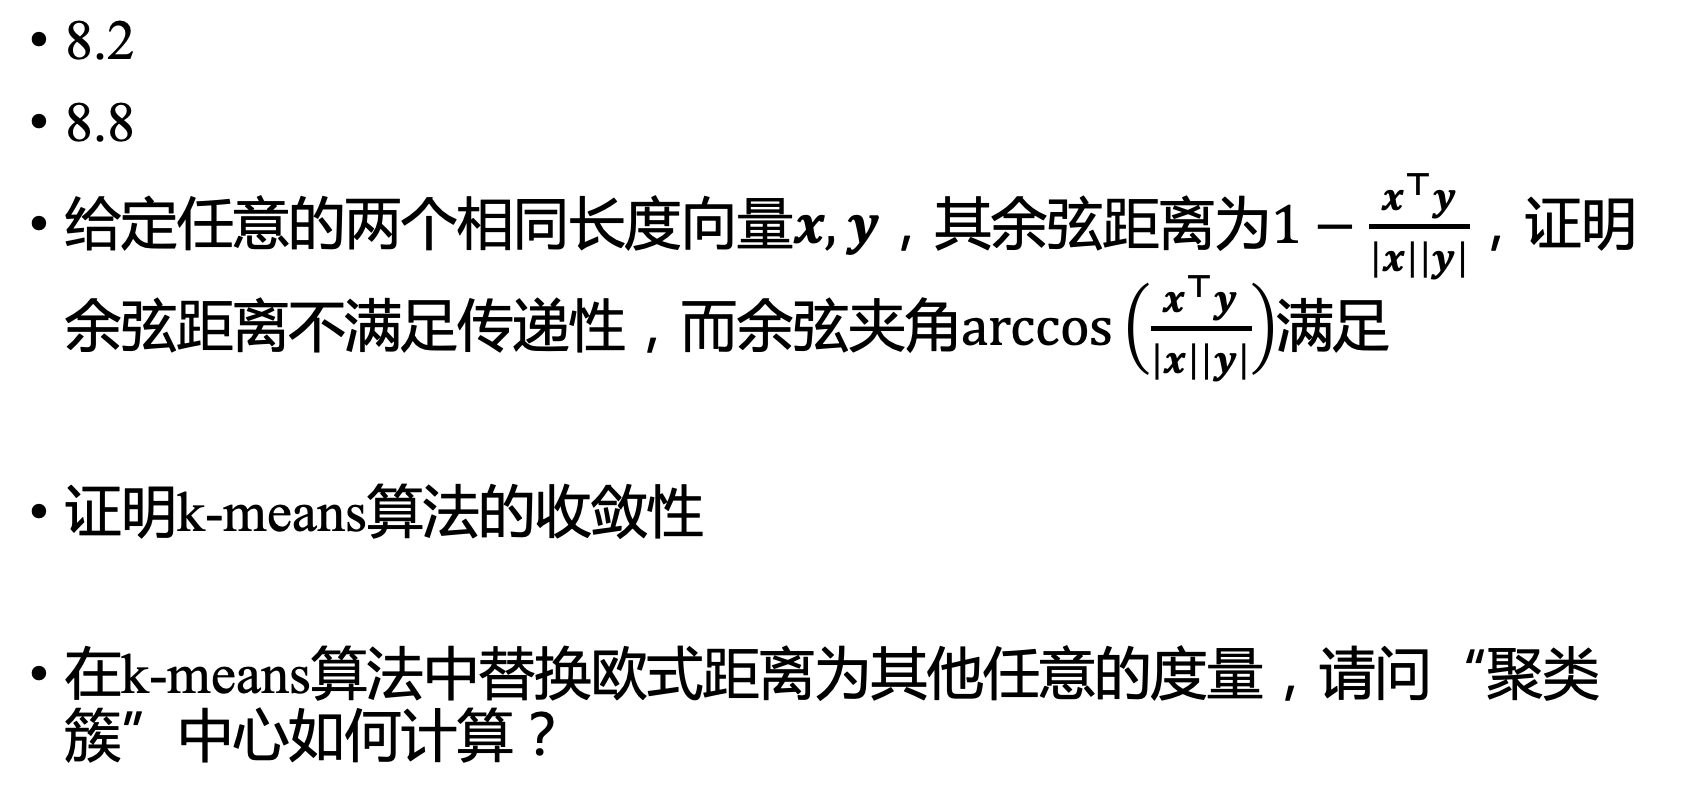
\includegraphics[scale=0.425]{hw8&9.png}
  % \caption{}
  \label{f8}
\end{figure}



\subsection{}

式(8.5)
\begin{equation*}
  \ell_{\exp }(H \mid \mathcal{D})=\mathbb{E}_{\boldsymbol{x} \sim \mathcal{D}}\left[e^{-f(\boldsymbol{x}) H(\boldsymbol{x})}\right]
\end{equation*}

由式(8.4)
\begin{equation*}
  H(\boldsymbol{x})=\sum_{t=1}^{T} \alpha_{t} h_{t}(\boldsymbol{x})
\end{equation*}

再由式(8.11)
\begin{equation*}
  \alpha_{t}=\frac{1}{2} \ln \left(\frac{1-\epsilon_{t}}{\epsilon_{t}}\right)
\end{equation*}
可以看出分类器的权重只与分类器的错误率负相关。

对于式(8.5)的情况时,由于 $ f(x) \in \{+1,-1\} $,$H(x)$为实数,当两者同号时,
有$f(x)H(x)>0$,此时,$e^{-f(x)H(x)} = e^{-|H(x)|} < 1$,$|H(x)|$越大损失函数越小;
两者异号时,有$f(x)H(x)<0$,此时,$e^{-f(x)H(x)} = e^{|H(x)|} > 1$,$|H(x)|$越大损失函数越大。
且由于指数函数的性质,在两个区间的时候损失函数都是单调的。

由此,当使用任意损失函数$\ell(-f(x)H(x))$,且对于$H(x)$在区间$[-\infty,\delta](\delta>0)$单调递减的情况,
仍然满足损失函数是分类任务原本的0 / 1 损失函数的 一致的替代损失函数。



\subsection{}

MultiBoosting由于集合了Bagging,Wagging,AdaBoost,可以有效的降低误差和方差,特别是误差,但是训练成本和预测成本都会显著增加。

Iterative Bagging相比Bagging会降低误差,但是方差上升。由于Bagging本身就是一种降低方差的算法,所以Iterative Bagging相当于Bagging与单分类器的折中。





% -------------------------------section分割线-------------------------------------------

\section{HW9}

\subsection{}

\begin{itemize}
  \item 余弦距离不满足传递性:
\end{itemize}

不妨令空间中三个点的坐标如下:

$$ x = (1,0), y = (0,1), z = (\frac{\sqrt{2}}{2},\frac{\sqrt{2}}{2}) $$
则,余弦距离有:
$$ d(x,y) = 1, d(x,z) = 1-\frac{\sqrt{2}}{2}, d(z,y) = 1-\frac{\sqrt{2}}{2} $$
此时,$ d(x,z)+d(y,z) < d(x,y) $.
故余弦距离不满足传递性。

\begin{itemize}
  \item 余弦夹角满足传递性:
\end{itemize}

证明:$$ \arccos \left(\frac{\left(\boldsymbol{x}^{\top} \boldsymbol{y}\right)}{|\boldsymbol{x}||\boldsymbol{y}|}\right) \leq \arccos \left(\frac{\left(\boldsymbol{x}^{\top} \boldsymbol{z}\right)}{|\boldsymbol{x}||\boldsymbol{z}|}\right)+\arccos \left(\frac{\left(\boldsymbol{z}^{\top} \boldsymbol{y}\right)}{|\boldsymbol{z}||\boldsymbol{y}|}\right) $$

两侧同时取cos,由于在区间$[0,\pi]$上单调递减,于是在该区间有:
\begin{equation*}
  \begin{aligned}
    \frac{\left(\boldsymbol{x}^{\top} \boldsymbol{y}\right)}{|\boldsymbol{x} \| \boldsymbol{y}|} & \geq \cos \left(\arccos \left(\frac{\left(\boldsymbol{x}^{\top} \boldsymbol{z}\right)}{|\boldsymbol{x} \| \boldsymbol{z}|}\right)+\arccos \left(\frac{\left(\boldsymbol{z}^{\top} \boldsymbol{y}\right)}{|\boldsymbol{z}||\boldsymbol{y}|}\right)\right)                                                                                                                                                                                                      \\
                                                                                                 & = \frac{\left(\boldsymbol{x}^{\top} \boldsymbol{z}\right)}{|\boldsymbol{x} \| \boldsymbol{z}|} * \frac{\left(\boldsymbol{z}^{\top} \boldsymbol{y}\right)}{|\boldsymbol{z}||\boldsymbol{y}|}-\sqrt{\left(1-\left(\frac{\left(\boldsymbol{x}^{\top} \boldsymbol{z}\right)}{|\boldsymbol{x} \| \boldsymbol{z}|}\right)^{2}\right) *\left(1-\left(\frac{\left(\boldsymbol{z}^{\top} \boldsymbol{y}\right)}{|\boldsymbol{z} \| \boldsymbol{y}|}\right)^{2}\right)} \\
                                                                                                 & = \frac{\boldsymbol{x}^{\top}\left(\boldsymbol{z} \boldsymbol{z}^{\top}\right) \boldsymbol{y}}{|\boldsymbol{x}\|\boldsymbol{z}|| \boldsymbol{z}\| \boldsymbol{y}|}-\sqrt{\left(1-\left(\frac{\left(\boldsymbol{x}^{\top} \boldsymbol{z}\right)}{|\boldsymbol{x} \| \boldsymbol{z}|}\right)^{2}\right) *\left(1-\left(\frac{\left(\boldsymbol{z}^{\top} \boldsymbol{y}\right)}{|\boldsymbol{z} \| \boldsymbol{y}|}\right)^{2}\right)}                          \\
                                                                                                 & = \frac{\left(\boldsymbol{x}^{\top} \boldsymbol{y}\right)}{|\boldsymbol{x} \| \boldsymbol{y}|}-\sqrt{\left(1-\left(\frac{\left.\boldsymbol{x}^{\top} \boldsymbol{z}\right)}{|\boldsymbol{x} \| \boldsymbol{z}|}\right)^{2}\right) *\left(1-\left(\frac{\left(\boldsymbol{z}^{\top} \boldsymbol{y}\right)}{|\boldsymbol{z}||\boldsymbol{y}|}\right)^{2}\right)}
    % &\leq \frac{\left(\boldsymbol{x}^{\top} \boldsymbol{y}\right)}{|\boldsymbol{x} \| \boldsymbol{y}|}
  \end{aligned}
\end{equation*}
由于:$ \sqrt{\left(1-\left(\frac{\left.\boldsymbol{x}^{\top} \boldsymbol{z}\right)}{|\boldsymbol{x} \| \boldsymbol{z}|}\right)^{2}\right) *\left(1-\left(\frac{\left(\boldsymbol{z}^{\top} \boldsymbol{y}\right)}{|\boldsymbol{z}||\boldsymbol{y}|}\right)^{2}\right)} \geq 0 $,
故不等式得证。
余弦夹角满足传递性。



\subsection{}

\begin{quotation}
  \item 证明k-means算法的收敛性
\end{quotation}

即证明:
\begin{equation*}
  \min J\left(u_{1}, u_{2}, \ldots u_{k}\right)=1 / 2 \sum_{i=1}^{m} \sum_{j=1}^{k}\left(x_{i}-u_{j}\right)^{2}
\end{equation*}
1)单调;2)有界。

\begin{enumerate}
  \item 单调
        \begin{enumerate}
          \item 更新m个点的归属类别:将m个点归属到已有的k个中心,其中的判定就是离哪个中心点近,就归属到那一类,此时损失函数为$ J_0\left(u_{1}, u_{2}, \ldots u_{k}\right) $.
                在中心确定的情况下,如果不归属到最近的中心,归属到其他中心,此刻损失函数假设为$ J_1\left(u_{1}, u_{2}, \ldots u_{k}\right) $,
                一定有$ J_0 \leq J_1 $. (假如其中m-1个点都归属到最近的中心了,某一个点没有归属到最近中心,那么如果把这个点放到最近的那个中心,损失函数就会降低)
          \item 假设第一个类别有$N_1$个点,中心为$u_j$,这个类别的损失函数部分为$1 / 2 \sum_{i=1}^{N_{1}}\left(x_{i}-u_{1}\right)^{2}$,且有:
                $ 1 / 2 \sum_{i=1}^{N_{1}}\left(x_{i}-u_{1}\right)^{2} \geq 1 / 2 \sum_{i=1}^{N_{1}}\left(x_{i}-x_{\text {ave }}\right)^{2} \text { 其中 } x_{\text {ave }} $,
                $x_{ave}$为其均值中心。固定归属类别,通过把均值中心作为类别中心,降低了$J$
        \end{enumerate}
  \item 有界

        $J\left(u_{1}, u_{2}, \ldots u_{k}\right) \geq 0$
\end{enumerate}
故,单调,有界,收敛。



\subsection{}

\begin{quotation}
  在k-means算法中替换欧氏距离为其他任意的度量,请问聚类簇“中心”如何计算?
\end{quotation}

直接进行平均计算得到的均值是符合欧几里得距离定义下的均值的定义的,但是并不一定符合其它距离计算公式。
不同距离的定义方式需要设计一套单独的“均值”的定义方式进行聚类簇“中心”的计算。
若损失函数是凸的,则直接对其求梯度并令其等于0,可得到聚类中心。同时,很可能完全定义不出来,如曼哈顿距离。





% -------------------------------section分割线-------------------------------------------

\section{HW10}

\begin{figure}[H]
  \centering
  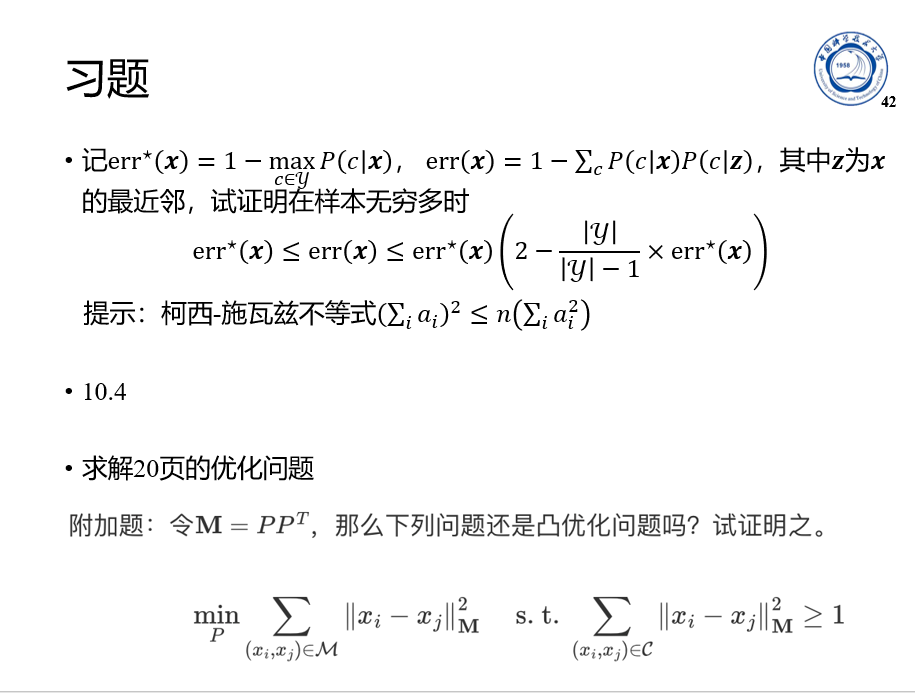
\includegraphics[scale=0.325]{hw10.png}
  % \caption{}
  \label{f10}
\end{figure}



\subsection{}

由题可知:
\begin{equation*}
  \operatorname{err}^{\star}(\boldsymbol{x})=1-\max _{c \in Y} P(c \mid \boldsymbol{x})
\end{equation*}
\begin{equation*}
  \operatorname{err}(\boldsymbol{x})=1-\sum_{c} P(c \mid \boldsymbol{x}) P(c \mid \boldsymbol{z})
\end{equation*}

要证$\operatorname{err}^{\star}(\boldsymbol{x}) \leq \operatorname{err}(\boldsymbol{x})$

即证$\max _{c \in Y} P(c \mid \boldsymbol{x}) \geq \sum_{c} P(c \mid \boldsymbol{x}) P(c \mid \boldsymbol{z})$

\begin{equation*}
  \begin{aligned}
    \sum_{c} P(c \mid \boldsymbol{x}) P(c \mid \boldsymbol{z}) & \approx \sum_{c} P(c \mid \boldsymbol{x})^2                                    \\
                                                               & \leq \max_{c \in Y}  P(c \mid \boldsymbol{x}) \sum_c  P(c \mid \boldsymbol{x}) \\
                                                               & = \max _{c \in Y} P(c \mid \boldsymbol{x})
  \end{aligned}
\end{equation*}
得证.

要证$\operatorname{err}(\boldsymbol{x}) \leq \operatorname{err}^{\star}(\boldsymbol{x})\left(2-\frac{|\mathcal{Y}|}{|\mathcal{Y}|-1} \times \operatorname{err}^{\star}(\boldsymbol{x})\right)$

\begin{equation*}
  \begin{aligned}
    \operatorname{err}(x) & =1- \sum_x P^{2}(c \mid x)                                                                                        \\
                          & =\left(2-\operatorname{err}^{\star}(x)\right) \operatorname{err}^{\star}(x)-\sum_{c \mid c^\star} P^{2}(c \mid x)
  \end{aligned}
\end{equation*}

由Cauchy不等式:
\begin{equation*}
  \sum_{c \mid c^\star} P^{2}(c \mid x) \geq \frac{1}{|\mathcal{Y}|}(1-P(c^\star \mid x))^2 = \frac{1}{|\mathcal{Y}|}\operatorname{err}^{\star}(\boldsymbol{x})^2
\end{equation*}

即:$\operatorname{err}(\boldsymbol{x}) \leq \operatorname{err}^{\star}(\boldsymbol{x})\left(2-\frac{|\mathcal{Y}|}{|\mathcal{Y}|-1} \times \operatorname{err}^{\star}(\boldsymbol{x})\right)$



\subsection{}

\begin{mdframed}[hidealllines=true,backgroundcolor=shadecolor]
  \begin{verbatim}
  在实践中,协方差矩阵XX^T的特征值分解常由中心化后的样本矩阵X的奇异值分解代
  替,试述其原因.
\end{verbatim}
\end{mdframed}

因为两者等价,下证明:

X的奇异值分解为:
$$ X=U \Sigma V^{T}, \quad X X^{T}=U \Sigma V^{T}\left(U \Sigma V^{T}\right)^{T}=U \Sigma V^{T} V \Sigma^{T} U^{T} $$
此时,$ V^TV=1, U^TU=1 $,故,
$$ X X^{T}=U \Sigma \Sigma^{T} U^{T}=U \Lambda U^{T} $$

X的特征值分解时,$ X^TX = P\Lambda P^T $, P=U则两者等价。

还有,用奇异值分解代替特征分解,节省了计算和存储的成本,且计算精度较高。



\subsection{}

\begin{framed}
  \begin{quotation}
    主成分分析—求解
    $$\max _{\boldsymbol{W}} \operatorname{tr}\left(\boldsymbol{W}^{T} \boldsymbol{X} \boldsymbol{X}^{T} \boldsymbol{W}\right) \quad \text { s.t. } \boldsymbol{W}^{T} \boldsymbol{W}=\boldsymbol{I}_{d^{\prime}}$$
    使用拉格朗日乘子法可得
    $$ X X^{T} W=\Lambda W $$
  \end{quotation}
\end{framed}

由题得:拉格朗日函数为:
$$ L(w, \theta)=\operatorname{tr}\left(W^{T} X X^{T} W\right)-\operatorname{tr}\left(\theta^{T}\left(w^{T} W-I\right)\right) $$
其中,$\theta$ 乘子矩阵。考虑其中前d'个最大的特征值,令$ \theta = diag(\lambda_1,\Lambda_2,\dots,\lambda_{d'}) $
则:
\begin{equation*}
  \begin{aligned}
    \frac{\partial L (W, \theta)}{\partial W} & =\frac{\partial\left(\operatorname{tr}\left(W^{T} X X^{T} W\right)\right.}{\partial W}-\frac{\partial}{\partial W}\left(\operatorname{tr}\left(\theta^{T}\left(W^{T} W-I\right)\right)\right) \\
                                              & =2 X X^{T} W-W \theta-W \theta^{T}                                                                                                                                                            \\
                                              & =2 X X^{T} W-2 W \theta
  \end{aligned}
\end{equation*}
为0时,有
$$ X X^{T} W = 2 W \theta $$
代回,有:
\begin{equation*}
  \begin{aligned}
      & \max _{W} \operatorname{tr}\left(W^{T} X x^{T} W\right)   \\
    = & \max _{W} \sum_{i=1}^{d^{\prime}} W_{i}^{T} X x^{T} W_{i} \\
    = & \max _{i=1} \sum_{i}^{\prime} \lambda_{i} W_{i}^{T} W_{i} \\
    = & \max ^{x} \sum_{i=1}^{d^{\prime}} \lambda_{i}
  \end{aligned}
\end{equation*}



% -------------------------------section分割线-------------------------------------------

\section{HW11}

\begin{figure}[H]
  \centering
  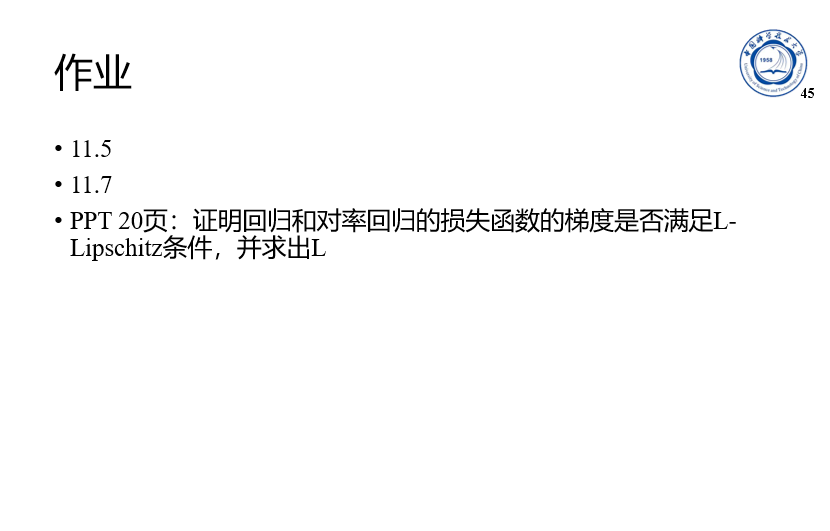
\includegraphics[scale=0.375]{hw11.png}
  % \caption{}
  \label{f11}
\end{figure}



\subsection{}

\begin{mdframed}[hidealllines=true,backgroundcolor=shadecolor]
  \begin{verbatim}
    结合图11.2,试举例说明 L1 正则化在何种情形下不能产生稀疏解.
  \end{verbatim}
\end{mdframed}

\begin{figure}[H]
  \centering
  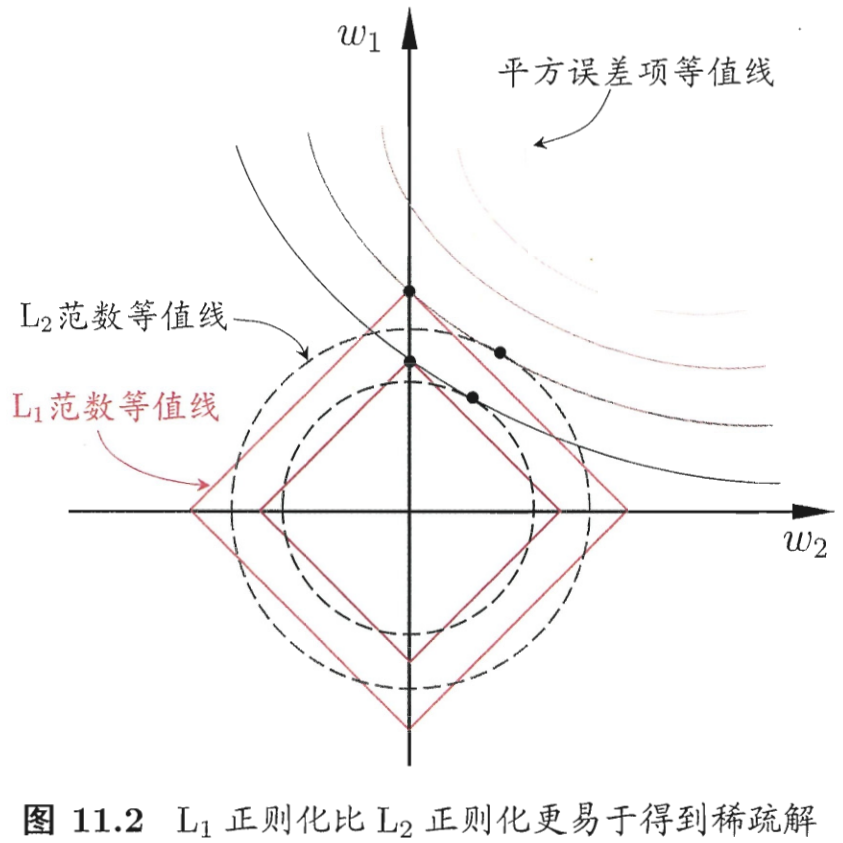
\includegraphics[scale=0.3]{./引用/11.2.png}
  % \caption{}
  \label{f11.2}
\end{figure}

L1正则化之所以可以产生稀疏解,主要是因为平方误差项等值线与L1等值线的第一个交点位于坐标轴上,如书上图11.2所示,当平方误差项等值线的曲率比较大时,就会导致其与L1等值线的第一个交点不再位于坐标轴上,此时就无法产生稀疏解。



\subsection{}

\begin{mdframed}[hidealllines=true,backgroundcolor=shadecolor]
  \begin{verbatim}
    试述直接求解 L0 范数正则化会遇到的困难.
  \end{verbatim}
\end{mdframed}

L0 范数是不连续的,而且是非凸函数,无法通过优化直接求解,必须采用遍历的方式,因此导致这个问题是个NP难问题。



\subsection{}

\subsubsection{}

回归:
$$ f(w) = \Vert Xw-y \Vert^2  $$
故,
$$ \nabla f(w) = 2X^T(Xw-y) $$
任取$w_1, w_2$,
\begin{equation*}
  \begin{aligned}
    \left\|\nabla f(w_1)-\nabla f(w_2) \right\|_2 & = 2 \left\|X^T(Xw_1-y)-X^T(Xw_2-y) \right\|_2            \\
                                                  & = 2 \left\|X^T X(w_1-w_2) \right\|_2                     \\
                                                  & \leq 2 \left\|X^T X \right\|_2 \left\|w_1-w_2 \right\|_2
  \end{aligned}
\end{equation*}
则,满足L-Lipschitz条件,且$ \mathcal{L} = 2 \left\|X^T X \right\|_2 = 2 \left\| X \right\|_2^2 $


\subsubsection{}

对率回归:
$$ f(w) = \sum_{i=1}^{m} (-yw^{T}x_i + \ln (1+e^{w^{T}x_i})) $$
故,
$$ \nabla f(w) = -\sum_{i=1}^{m} (y_i - \frac{e^{w^{T}x_i}}{1+e^{w^{T}x_i}})x_i $$
任取$w_1, w_2$,
\begin{equation*}
  \begin{aligned}
    \left\|\nabla f(w_1)-\nabla f(w_2) \right\|_2 & = \left\|(-\sum_{i=1}^{m} (y_i - \frac{e^{w_1^{T}x_i}}{1+e^{w_1^{T}x_i}})x_i) - (-\sum_{i=1}^{m} (y_i - \frac{e^{w_2^{T}x_i}}{1+e^{w_2^{T}x_i}})x_i) \right\|_2 \\
                                                  & = \left\|\sum_{i=1}^{m} (\frac{e^{w_1^{T}x_i}}{1+e^{w_1^{T}x_i}}-\frac{e^{w_2^{T}x_i}}{1+e^{w_2^{T}x_i}})x_i \right\|_2
  \end{aligned}
\end{equation*}

令$ g(\alpha) = \frac{e^{\alpha}}{1+e^{\alpha}} $
$$ \nabla g(\alpha)=\frac{e^{\alpha}}{\left(1+e^{\alpha}\right)^{2}} \geq 0 ,~~  \nabla^{2} g(\alpha)=-\frac{e^{\alpha}\left(e^{\alpha}-1\right)}{\left(1+e^{\alpha}\right)^{3}} $$
二阶导数为0时,$\alpha=0$,一阶导数在此处取得极大值$\frac{1}{4}$.
\begin{equation*}
  \begin{aligned}
    \| g(\alpha)-g(\beta) \|_{2} & =\left\|\frac{e^{\alpha}}{1+e^{\alpha}}-\frac{e^{\beta}}{1+e^{\beta}}\right\|_{2} \\
                                 & =\|\nabla(\xi)(\alpha-\beta)\|_{2} \quad \xi \in(\alpha, \beta)                   \\
                                 & \leq \frac{1}{4}\|\alpha-\beta\|_{2}
  \end{aligned}
\end{equation*}
故,
\begin{equation*}
  \begin{aligned}
    \left\|\nabla f\left(w_1\right)-\nabla f(w_2)\right\|_{2} & \leq \frac{1}{4}\left\|\sum\left(w_2^{T} x_{i}-w_2^{T} x_{i}\right) x_{i}\right\|_{2} \\
                                                              & =\frac{1}{4}\left\|x^{T} x\left(w_1-w_2\right)\right\|_{2}                            \\
                                                              & \leq \frac{1}{4}\left\|x^{T} x\right\|_{2}\left\|w_1-w_2\right\|_{2}
  \end{aligned}
\end{equation*}

则,满足L-Lipschitz条件,且$ \mathcal{L} = \frac{1}{4} \left\|X^T X \right\|_2 = \frac{1}{4} \left\| X \right\|_2^2 $




% -------------------------------section分割线-------------------------------------------

\section{HW12}

无



% -------------------------------section分割线-------------------------------------------

\section{HW13}

无



% -------------------------------section分割线-------------------------------------------

\section{HW14}

\begin{figure}[H]
  \centering
  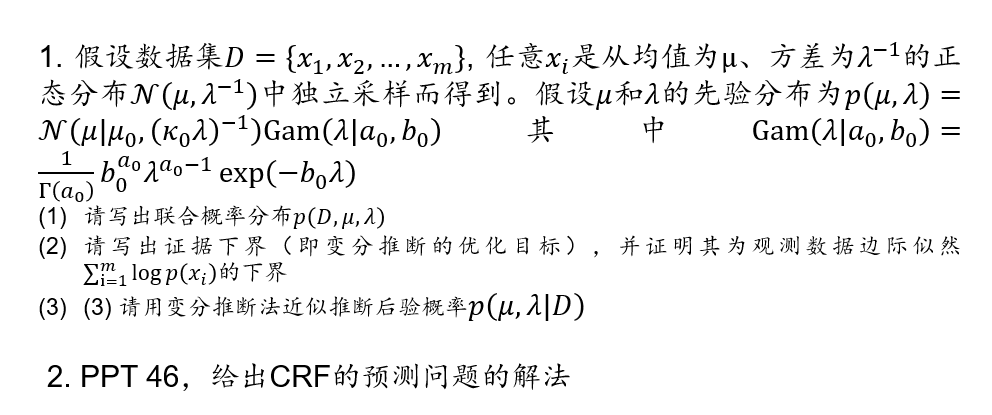
\includegraphics[scale=0.675]{hw14.png}
  % \caption{}
  \label{f:hw14}
\end{figure}



\subsection{}

\subsubsection{}

\begin{equation*}
  \begin{aligned}
    p\left(D, \mu, \lambda\right) & =p(\mu, \lambda) \cdot p(D \mid \mu, \lambda)                                                                                                                                                                                                                  \\
                                  & =p(\mu, \lambda) \cdot \prod_{i=1}^{m} p\left(x_{i} \mid \mu, \lambda\right)                                                                                                                                                                                   \\
                                  & =\frac{1}{\sqrt{2 \pi(\kappa_0\lambda)^{-1}}} \exp \left\{-\frac{1}{2(\kappa _0 \lambda)^{-1}}\left(\mu-\mu_{0}\right)^{2}\right\}                                                                                                                             \\
                                  & ~~~  \cdot  \frac{1}{\Gamma \left(a_{0}\right)} b_{0}^{a_{0}} \cdot \lambda^{a_{0}-1} \exp \left\{-b_{0} \lambda\right\} \cdot\left(\frac{\lambda}{2 \pi}\right)^{\frac{m}{2}} \exp \left\{-\frac{\lambda}{2} \sum_{i=1}^{m}\left(x_{i}-\mu\right)^{2}\right\}
  \end{aligned}
\end{equation*}


\subsubsection{}

由题可知,变分推断的目的是寻找一个参数的概率密度函数
\begin{equation*}
  q(z)~~\text{s.t.}~ q^*(z) = \mathop{\arg\min}\limits_{q(z)} KL\left(q(z)\| p(z|x)\right)
\end{equation*}
其中,KL散度为
$$ KL(q(z) \| p(z \mid x))=\mathbf{E} [\log q(z)]-\mathbf{E} [\log p(z, x)]+\log p(x) $$
再由于KL散度的非负性,
故可得到:
\begin{equation*}
  \begin{aligned}
    ELBO & = \mathbf{E} [\log p(z,x)]-\mathbf{E} [\log q(z)]                                                                                                                       \\
         & =\mathbf{E}_q [\log p(\lambda)] + \mathbf{E}_q [\log p(\mu|\lambda)] + \mathbf{E}_q[\log p(x|\mu,\lambda)] - \mathbf{E}_q[\log q(\lambda)] - \mathbf{E}_q [\log q(\mu)]
  \end{aligned}
\end{equation*}


\subsubsection{}

由题可得,
$$ \frac{\partial L}{\partial q_u(u)}=E_{\lambda}[\log p(\mu \mid \lambda)]+E_{\lambda}[\log p(D \mid \mu, \lambda)]-\log q(u)=0 $$
\begin{equation*}
  \begin{aligned}
    \log q(u) & =\frac{E[\lambda] \kappa_{0}}{-2}\left(\mu-\mu_{0}\right)^{2}-\frac{E[\lambda]}{2} \sum_{i=1}^{m}\left(x_{i}-\mu\right)^{2}                                                                                                    \\
              & =-\frac{E[x]}{2}\left[\left(\kappa_{0}+m\right) \mu^{2}+\sum_{i=1}^{m} x_{i}^{2}-2 \mu\left(\kappa_{0} \mu_{0}+m \bar{x}\right)\right]                                                                                         \\
              & =-\frac{E[\lambda]}{2}\left[\left(\kappa_{0}+m\right)\left(\mu-\frac{\kappa_{0} \mu_{0}+m \bar{x}}{\kappa_{0}+m}\right)^{2}+\sum_{i=1}^{m} x_{i}^{2}-\frac{\left(\kappa_{0} \mu_{0}+m \bar{x}\right)^{2}}{\kappa_{0}+m}\right]
  \end{aligned}
\end{equation*}
令$ \mu_m = \frac{\kappa_{0} \mu_{0}+m \bar{x}}{\kappa_{0}+m} $, $ \lambda_m = (\kappa_0+m)E[\lambda] $,
故可以看出:$ q_u^*(u) \sim \mathcal{N} (\mu \mid \mu_m, \lambda_m) $.

再由
$$ \frac{\partial L}{\partial q_{\lambda}(\lambda)}=E_{\mu}[\log p(D \mid \lambda, \mu)]+E_{\mu}[\log (\mu \mid \lambda)]+E_{\mu}[\log p(\lambda)]-\log q(\lambda)=0 $$
故
\begin{equation*}
  \begin{aligned}
    \log q^{*}(\lambda) & =-\frac{\lambda}{2} E_{\mu}\left[\kappa_{0}\left(\mu-\mu_{0}\right)^{2}+\sum_{i=1}^{m}\left(x_{i}-\mu\right)^{2}\right]+\left(a_{0}-1\right) \log \lambda-b_{0} \lambda+\frac{m+1}{2} \log \lambda \\
                        & =\left(a_{0}+\frac{m-1}{2}\right) \log \lambda-\left(b_{0}+\frac{1}{2} E_{\mu}\left[\kappa_{0}\left(\mu-\mu_{0}\right)^{2}+\sum_{i=1}^{m}\left(x_{i}-\mu\right)^{2}\right]\right) \lambda
  \end{aligned}
\end{equation*}
令$ a_{m}=a_{0}+\frac{m+1}{2} $, $ b_{m}=b_{0}+\frac{1}{2} E_{\mu}\left[\kappa_{0}\left(\mu-\mu_{0}\right)^{2}+\sum_{i=1}^{m}\left(x_{i}-\mu\right)^{2}\right] $,
\\可以看出:$ q^*(\lambda) \sim Gam(\lambda \mid a_m, b_m) $.

故,可以得到:
$ q^{*}(\mu, \lambda) \sim \mathcal{N} \left(\mu \mid N_{m}, \lambda_{m}^{-1}\right) Gam\left(\lambda \mid a_{m}, b_{m}\right)$

在无先验的情况下有:
\begin{equation*}
  \left\{
  \begin{array}{l}
    \mu_0 = a_0 = b_0 = \kappa_0 = 0 \\
    E[\lambda] = \frac{a_m}{b_m}     \\
    E[\mu] = \mu_m = \bar{x}         \\
    E[\mu^2] = \bar{x}^2+\frac{1}{m E[\lambda]}
  \end{array}
  \right.
\end{equation*}

可以解得:
$$ E[\lambda] = \frac{1}{E[x^2]-\bar{x}^2} = \frac{1}{\operatorname{Var}(x)} $$
$$ \lambda_m = \frac{m}{\operatorname{Var}(x)} $$
$$ b_m = b_{0}+\frac{1}{2} E_{\mu}\left[\kappa_{0}\mu-^{2}+\sum_{i=1}^{m}\left(x_{i}-\mu\right)^{2}\right] $$
记带入后的 $\lambda_m, b_m$ 为 $\lambda', b'$,可以得到:
$$ p(\mu, \lambda \mid D) \sim \mathcal{N} \left(\mu \mid \mu_{m}, \lambda^{\prime}\right) Gam\left(\lambda \mid a m, b^{\prime}\right) $$


\subsection{}

采用维特比算法,首先求出位置1的各个标记 j = 1,2,...,m 的非规范化概率:
$$ \delta_{1}(j)=\omega * F_{1}\left(y_{0}=\text { start, } y_{1}=j, x\right), \quad j=1,2, \ldots, m $$

由递推公式,求出位置i的各个标记l = 1,2,…,m的非规范化概率的最大值,同时记录非规范化概率最大值的路径:
$$ \delta_{i}(l)=\max _{1 \leq j \leq m}\left\{\delta_{i-1}(l)+\omega * F_{i}\left(y_{i-1}=j, y_{i}=l, x\right)\right\}, \quad l=1,2, \ldots, m  $$
$$ \Psi_{i}(l)=\arg \max _{1 \leq j \leq m}\left\{\delta_{i-1}(l)+\omega * F_{i}\left(y_{i-1}=j, y_{i}=l, x\right)\right\}, \quad l=1,2, \ldots, m $$

直到i = n时终止,此时求得非规范化概率的最大值为:
$$ \max _{y}(\omega * F(y, x))=\max _{1 \leq j \leq m} \delta_{n}(j) $$
以及最优路径的终点
$$ y_{n}^{*}=\max _{1 \leq j \leq m} \delta_{n}(j) $$
由此最优路径终点返回
$$ y_{i}^{*}=\Psi_{i+1}\left(y_{i+1}^{*}\right), \quad \mathrm{i}=\mathrm{n}-1, \mathrm{n}-2, \ldots, 1 $$
最终求得最优路径.








% \bibliographystyle{gbt7714-numerical}
% % \bibliographystyle{7714-author-year}
% \bibliographystyle{ieeetr}
% \bibliography{bibl}

\end{document}